\documentclass[a4paper, 12pt]{report}
%\usepackage{vntex}
\usepackage[english,vietnam]{babel}
\usepackage{pdfpages}
%\usepackage[utf8]{inputenc}
\usepackage[newfloat]{minted}
%\usepackage[utf8]{inputenc}
%\usepackage[francais]{babel}
\usepackage{a4wide,amssymb,epsfig,latexsym,multicol,array,hhline,fancyhdr}
\usepackage{booktabs}
\usepackage{lmodern}
\usepackage{eqparbox}
\usepackage{makecell, caption}
\usepackage[toc,page]{appendix}
\usepackage{diagbox}
\usepackage{amsmath}
\usepackage{amsfonts}
\usepackage{amssymb}
\usepackage{bm}
\usepackage{lastpage}
\usepackage{fourier}
\usepackage[lined,boxed,commentsnumbered]{algorithm2e}
\usepackage{enumerate}
\usepackage{colortbl}
%\usepackage{color}
\usepackage[usenames,dvipsnames]{color}
\usepackage{graphicx}							% Standard graphics package
\usepackage{array}
\usepackage{adjustbox}
\usepackage{indentfirst}
\usepackage{tabularx, caption}
\usepackage{multirow}
\usepackage[framemethod=tikz]{mdframed}% For highlighting paragraph backgrounds
\usepackage{multicol}
\usepackage{rotating}
\usepackage{graphics}
\usepackage{geometry}
\usepackage{setspace}
\usepackage{epsfig}
\usepackage{tikz}
\usepackage{listings}
\usetikzlibrary{arrows,snakes,backgrounds}
\usepackage{hyperref}
\usepackage{floatrow}
\usepackage{blindtext}
\usepackage{amsmath}
\usepackage{amsfonts}
\usepackage{fourier}
\usepackage{amssymb}
\usepackage[dvipsnames]{xcolor}
\usepackage{listings}
\usepackage{xcolor}
\usepackage{lineno, blindtext, amsmath, mathtools}
\providecommand{\phantomsection}{}
\newenvironment{preface}[1]{
  \vspace*{\stretch{1}}
  {\noindent \bfseries \Huge #1}
  \begin{center}
    \thispagestyle{plain}
    \phantomsection\addcontentsline{toc}{chapter}{#1}
  \end{center}
}{
  \vspace*{\stretch{7}}
}


%
\definecolor{codegreen}{rgb}{0,0.6,0}
\definecolor{codegray}{rgb}{0.5,0.5,0.5}
\definecolor{codepurple}{rgb}{0.58,0,0.82}
%\definecolor{backcolour}{rgb}{0,0.95,0.92}
%% Remember to load babel before loading this package or define the command \abstractname!
	  
\lstdefinestyle{mystyle}{
    backgroundcolor=\color{white},   
    commentstyle=\color{codegreen},
    keywordstyle=\color{magenta},
    numberstyle=\tiny\color{codegray},
    stringstyle=\color{codepurple},
    basicstyle=\ttfamily\footnotesize,
    breakatwhitespace=false,         
    breaklines=true,                 
    captionpos=b,                    
    keepspaces=true,                 
    numbers=left,                    
    numbersep=5pt,                  
    showspaces=false,                
    showstringspaces=false,
    showtabs=false,                  
    tabsize=2
}

\lstset{style=mystyle}
%Font size
\fontsize{10pt}{18pt}\selectfont
% \usepackage{vntex}
\usepackage{lineno, blindtext}
%\documentclass{book}
\hypersetup{
    colorlinks=true,
    linkcolor=black,
    urlcolor=black,
    }

\urlstyle{same}



%\hypersetup{urlcolor=blue,linkcolor=black,citecolor=black,colorlinks=true} 
%\usepackage{pstcol} 								% PSTricks with the standard color package
\newfloatcommand{capbtabbox}{table}[][\FBwidth]

\newtheorem{theorem}{{\bf Định lý}}
\newtheorem{property}{{\bf Tính chất}}
\newtheorem{proposition}{{\bf Mệnh đề}}
\newtheorem{corollary}[proposition]{{\bf Hệ quả}}
\newtheorem{lemma}[proposition]{{\bf Bổ đề}}
\newmdenv[linecolor=black,skipabove=\topsep,skipbelow=\topsep,
leftmargin=-5pt,rightmargin=-5pt,
innerleftmargin=5pt,innerrightmargin=5pt]{mybox}
%\everymath{\color{blue}}
%\usepackage{fancyhdr}

\def\thesislayout{	% A4: 210 × 297
	\geometry{
		a4paper,
		total={160mm,240mm},  % fix over page
		left=20mm,
		top=30mm,
	}
}
\thesislayout

\setlength{\headheight}{20pt}
\pagestyle{fancy}
\fancyhead{} % clear all header fields
\fancyhead[L]{
 \begin{tabular}{rl}
    \begin{picture}(20,10)(0,0)
    \put(0,-9){
\includegraphics[width=9.5mm, height=9.5mm]{picture/logoCSE.png}}
    %\put(0,-8){\epsfig{width=10mm,figure=hcmut.eps}}
   \end{picture}&
	%
\includegraphics[width=8mm, height=8mm]{hcmut.png} & %
	\begin{tabular}{l}
		\textcolor{black}{\textbf{\bf \ttfamily Ho Chi Minh City University of Technology}}\\
		\textcolor{black}{\textbf{\bf \ttfamily Faculty of Computer Science and Engineering}}
	\end{tabular} 	
 \end{tabular}
}
\fancyhead[R]{
	\begin{tabular}{l}
		\tiny \bf \\
		\tiny \bf 
	\end{tabular}  }
\fancyfoot{} % clear all footer fields
\fancyfoot[L]{\scriptsize \ttfamily Logic Design Project AY 2022-2023}
\fancyfoot[R]{\scriptsize \ttfamily Page {\thepage}/\pageref{LastPage}}
\renewcommand{\headrulewidth}{0.3pt}
\renewcommand{\footrulewidth}{0.3pt}


%%%
\def\@makechapterhead#1{%
  \vspace*{50\p@}%
  {\parindent \z@ \raggedright \normalfont \scshape
    \ifnum \c@secnumdepth >\m@ne
      \if@mainmatter
        \huge\bfseries \scshape \@chapapp\space \thechapter
        \par\nobreak
        \vskip 20\p@
      \fi
    \fi
    \interlinepenalty\@M
    \Huge \bfseries #1\par\nobreak
    \vskip 40\p@
  }}

\setcounter{secnumdepth}{4}
\setcounter{tocdepth}{1}
\makeatletter

\newcounter {subsubsubsection}[subsubsection]
\renewcommand\thesubsubsubsection{\thesubsubsection .\@arabic\c@subsubsubsection}
\newcommand\subsubsubsection{\@startsection{subsubsubsection}{4}{\z@}%
                                     {-3.25ex\@plus -1ex \@minus -.2ex}%
                                     {1.5ex \@plus .2ex}%
                                     {\normalfont\normalsize\bfseries}}
\newcommand*\l@subsubsubsection{\@dottedtocline{3}{10.0em}{4.1em}}
\newcommand*{\subsubsubsectionmark}[1]{}
\makeatother

%\definecolor{dkgreen}{rgb}{0,0.6,0}
\definecolor{gray}{rgb}{0.5,0.5,0.5}
\definecolor{mauve}{rgb}{0.58,0,0.82}


\usepackage{xcolor}
\usepackage{listings}

\lstset{frame=tb,
	language=Matlab,
	aboveskip=3mm,
	belowskip=3mm,
	showstringspaces=false,
	columns=flexible,
	basicstyle={\small\ttfamily},
	numbers=none,
	numberstyle=\tiny\color{gray},
	%keywordstyle=\color{blue},
	%commentstyle=\color{black},
	stringstyle=\color{mauve},
	breaklines=true,
	breakatwhitespace=true,
	tabsize=3,
	numbers=left,
	stepnumber=1,
	numbersep=1pt,    
	firstnumber=1,
	numberfirstline=true
}
\usepackage{scrextend}
\changefontsizes{13pt}
\usepackage{biblatex}
\usepackage[
    backend=biber,
    style=ieee,
  ]{biblatex}
\addbibresource{file.bib}
\begin{document}

\begin{titlepage}
\begin{center}
\textcolor{black}{\textbf{\large VIETNAM NATIONAL UNIVERSITY HO CHI MINH CITY}} \\
\textcolor{black}{\textbf{ \large HO CHI MINH CITY UNIVERSITY OF TECHNOLOGY}}\\
\textcolor{black}{\textbf{\large FACULTY OF COMPUTER SCIENCE AND ENGINEERING}}\\
-----------------------------------------
\end{center}

\vspace{1cm}

\begin{figure}[h!]
\begin{center}

\includegraphics[width=4.7cm]{3_Logo_BK.png}
\end{center}
\end{figure}

\vspace{0.7cm}


\begin{center}
\begin{tabular}{c}
	\multicolumn{1}{c}{\textcolor{black}{\textbf{{\large LOGIC DESIGN PROJECT REPORT}}}}\\
    ~~\\
    \textbf{{\textcolor{black}{\LARGE FPGA-BASED IMPLEMENTATION FOR }}}\\
    
    \textbf{\LARGE MACHINE LEARNING APPLICATION}\\
    \textbf{\LARGE AND CONVOLUTION COMPUTING SIMULATION}\\
    \\
    \large Major: Computer Engineering
\end{tabular}
\end{center}

\vspace{1.2cm}
\hspace{5.7cm}\textbf{LOGIC DESIGN PROJECT COMMITEE 3}
\begin{table}[h]
\begin{tabular}{rll}
\hspace{5cm}
& \textbf{INSTRUCTOR:} &\textbf{PHAM QUOC CUONG}\\
& & \textbf{PHAM DINH TRUNG}\\
\\
& \textbf{STUDENTS:} & \textbf{LE NGOC MINH THU }\\ 
& &\textbf{BUI ANH KHOA}\\
& &\textbf{NGUYEN PHAN ANH TUAN }

\end{tabular}
\end{table}
\vspace{1cm}
\begin{center}
{\textcolor{black}{\footnotesize Winter Semester, AY 2022-2023}}
\end{center}
\end{titlepage}

\begin{preface}{Acknowledgements}

  At first, we would like to express our gratitude to \textit{Associate Professor Pham Quoc Cuong} for supporting and creating opportunities for us to join in scientific research. 
  
  Thank you, \textit{Pham Dinh Trung}, for your enthusiasm of closely following our report process, helping us build background knowledge and also broaden our mindsets about semiconductor industry.
  
  Moreover, we would like to extend our special thanks to our two other teammates, \textit{Huynh Trung Nhat} and \textit{Le Tu Quan} for you guys' spirits which bring us a lot of supportive motivation to complete this project.

  Besides, our progress cannot going well without support from \textit{Tran Hoang Quoc Bao} and \textit{Mr Huynh Phuc Nghi} in CELab for helping us with technical problems and try to encouraging us with our chosen path.

  Thank you for all.
\end{preface}

%\begin{preface}{Abstract}
  Add your abstract here.
\end{preface}



\newpage
\tableofcontents
\newpage
\phantomsection\addcontentsline{toc}{chapter}{\listtablename}
\listoftables


\cleardoublepage
\phantomsection\addcontentsline{toc}{chapter}{\listfigurename}
\listoffigures

\mainmatter%
\chapter{Switches, Lights, and Multiplexers}

\section{Part I }
\begin{itemize}
    \item [] \textbf{REQUIREMENT}
        \begin{enumerate}
            \item Create a new Quartus project for your circuit. Select the target chip that corresponds to your DE-series board. Refer to Table 1 for a list of devices.
            \item Create a Verilog module for the code in Figure 1 and include it in your project.
            \item Include in your project the required pin assignments for your DE-series board, as discussed above. Compile the project.
            \item Download the compiled circuit into the FPGA chip by using the Quartus Programmer tool (the procedure for using the Programmer tool is described in the tutorial Quartus Introduction). Test the functionality of the circuit by toggling the switches and observing the LEDs.
        \end{enumerate}
    \item [] \textbf{SOLUTION}
            \begin{lstlisting}[language=verilog]
module part2(out, X, Y,S);
    output	[3:0]out;
    input		[3:0]X,Y;
    input		S;
    
    assign out = ({4{S}}&X) | ({4{~S}}&Y);
endmodule
            \end{lstlisting}
             \begin{figure}[h]
                \centering
                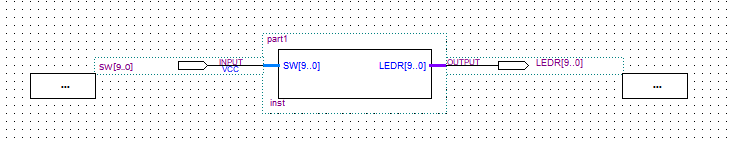
\includegraphics[scale = 0.9]{source/picture/Lab1/Lab1_1.png}
                \caption{Schematic for part 1}
            \end{figure}
\end{itemize}
\clearpage
\section{Part II }
\begin{itemize}
    \item [] \textbf{REQUIREMENT}
        \begin{enumerate}
            \item Create a new Quartus project for your circuit.
            \item Include your Verilog file for the four-bit wide 2-to-1 multiplexer in your project. Use switch $SW_9$ as the s input, switches $SW_{3-0}$ as the X input and $SW_{7-4}$ as the Y input. Display the value of the input s on $LEDR_9$, connect the output M to $LEDR_{3-0}$, and connect the unused LEDR lights to the constant value 0.
            \item Include in your project the required pin assignments for your DE-series board. As discussed in Part I, these assignments ensure that the ports of your Verilog code will use the pins on the FPGA chip that are connected to the SW switches and LEDR lights.
            \item Compile the project, and then download the resulting circuit into the FPGA chip. Test the functionality of the four-bit wide 2-to-1 multiplexer by toggling the switches and observing the LEDs
        \end{enumerate}
    \item [] \textbf{SOLUTION}
        \begin{lstlisting}[language= verilog]
module part2(out, X, Y,S);
	output	[3:0]out;
	input		[3:0]X,Y;
	input		S;
	
	assign out = ({4{S}}&X) | ({4{~S}}&Y);
	
endmodule
        \end{lstlisting}
        \begin{figure}[h]
            \centering
            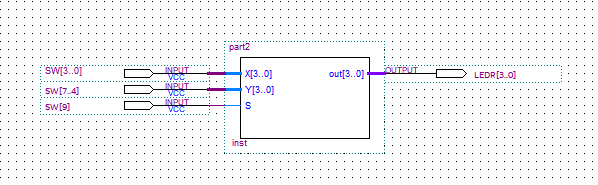
\includegraphics[scale =0.9]{source/picture/Lab1/Lab1_2.png}
            \caption{Schematic for part 2}
        \end{figure}
\end{itemize}
\clearpage
\section{Part III }
\begin{itemize}
    \item [] \textbf{REQUIREMENT}
        \begin{enumerate}
            \item Create a new Quartus project for your circuit.
            \item Create a Verilog module for the two-bit wide 4-to-1 multiplexer. Connect its select inputs to switches $SW_{9-8}$, and use switches $SW_{7-0}$ to provide the four 2-bit inputs U to X. Connect the output M to the red lights $LEDR_{1-0}$.
            \item Include in your project the required pin assignments for your DE-series board. Compile the project.
            \item Download the compiled circuit into the FPGA chip. Test the functionality of the two-bit wide 4-to-1 multiplexer by toggling the switches and observing the LEDs. Ensure that each of the inputs U to X can be properly selected as the output M.
        \end{enumerate}
    \item [] \textbf{SOLUTITON}
        \begin{lstlisting}[language = verilog]
module part3(M,U,V,W,X,S_1,S_0);
    input 	[1:0]U,V,W,X;
    input		S_1,S_0;
    output	[1:0]M;
    
    assign 	M= ({2{S_0&S_1}}&X)|
                    ({2{~S_0&S_1}}&W)|
                    ({2{S_0&~S_1}}&V)|
                    ({2{~S_0&~S_1}}&U);
	
endmodule
        \end{lstlisting}
        \begin{figure}[h]
            \centering
            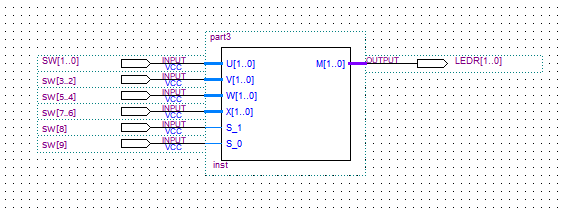
\includegraphics[width = \textwidth]{source/picture/Lab1/Lab1_3.png}
            \caption{Schemactic for part 3}
        \end{figure}
    
\end{itemize}
\clearpage
\section{Part IV }
\begin{itemize}
    \item [] \textbf{REQUIREMENT}
    \begin{enumerate}
        \item The objective of this part is to display a character on a 7-segment display. This decoder produces seven outputs that are used to display a character on a 7-segment display. Table 2 lists the characters that should be displayed for each valuation of c1c0 for your DE-series board.
        \item Note that in some cases the ‘blank’ character is selected for code 11. The seven segments in the display are identified by the indices 0 to 6 shown in the figure. Each segment is illuminated by driving it to the logic value 0. You are to write a Verilog module that implements logic functions to activate each of the seven segments.
    \end{enumerate}    
        \begin{figure}[h]
            \centering
            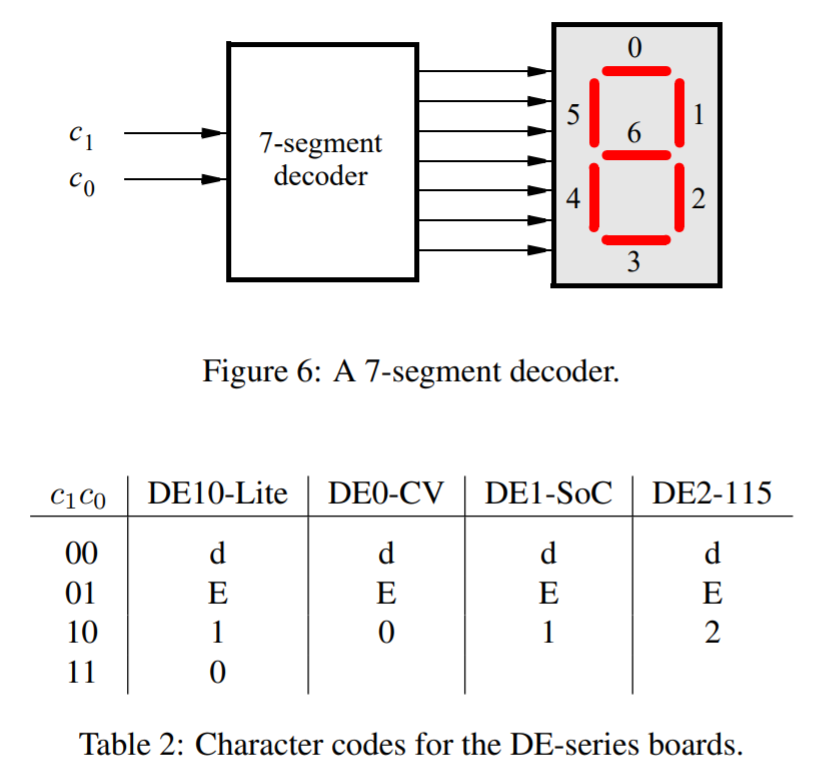
\includegraphics[scale =0.4]{source/picture/Lab1/1-4.png}
        \end{figure}
    \item [] \textbf{SOLUTION}
        \begin{lstlisting} [language = verilog]
module  part4(OUT,C_IN);
    input 	[1:0]C_IN;
    output	[6:0]OUT;
    
    assign 	OUT = (C_IN==0) ? 7'b0100001: 
                  (C_IN==1) ? 7'b0000110: 
                  (C_IN==2) ? 7'b0100100:7'b1111011;
endmodule
        \end{lstlisting}
        \begin{figure}[h]
            \centering
            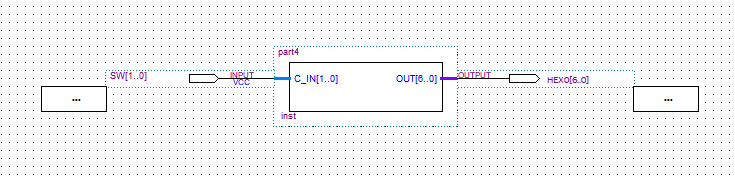
\includegraphics[width=\textwidth]{source/picture/Lab1/Lab1_4.png}
            \caption{Schemtatic for part 4}
        \end{figure}
\end{itemize}

\clearpage
\section{Part V }
\begin{itemize}
    \item [] \textbf{REQUIREMENT}
        \begin{enumerate}
            \item Consider the circuit shown in Figure 7. It uses a two-bit wide 4-to-1 multiplexer to enable the selection of four characters that are displayed on a 7-segment display. Using the 7-segment decoder from Part IV this circuit can display the characters d, E, 0, 1, 2, or 'blank' depending on your DE-series board. The character codes are set according to Table 2 by using the switches SW7-0, and a specific character is selected for display by setting the switches $SW_{9-8}$.
            \item Note that we have used the circuits from Parts III and IV as subcircuits in this code. The purpose of your circuit is to display any word on the four 7-segment displays that is composed of the characters in Table 2, and be able to rotate this word in a circular fashion across the displays when the switches SW9-8 are toggled. As an example, if the displayed word is dE10, then your circuit should produce the output patterns illustrated in Table 3.
        \end{enumerate}
        \begin{figure}[h]
            \centering
            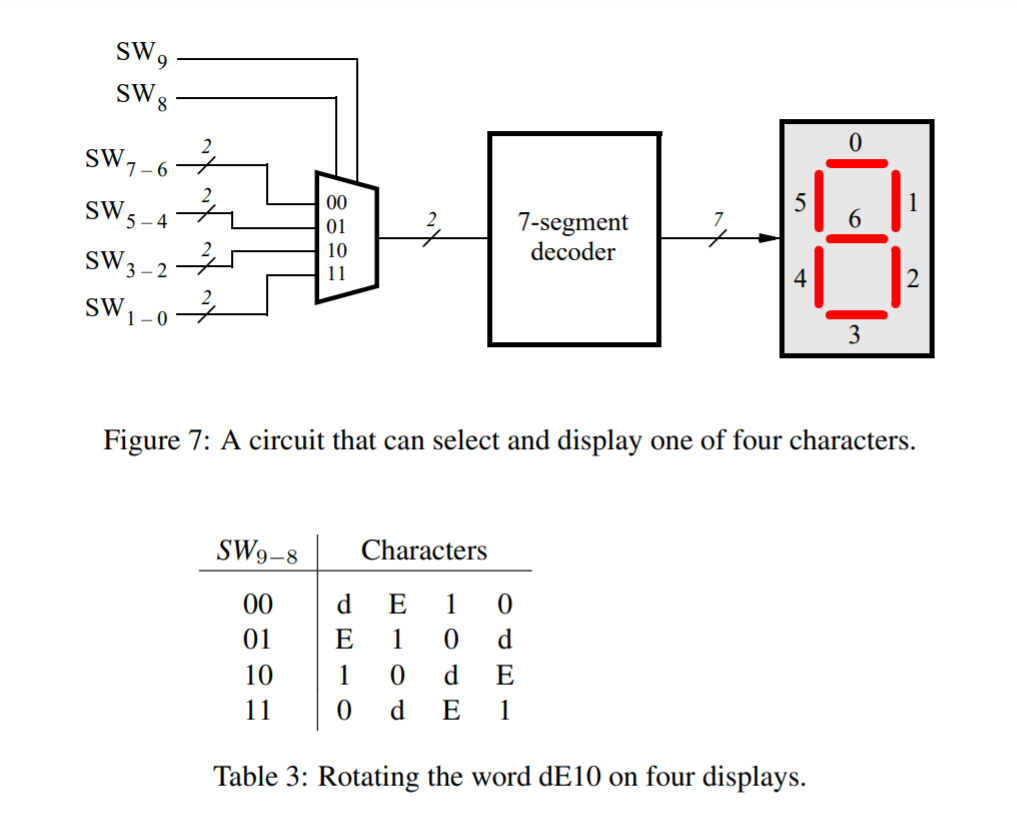
\includegraphics[scale =0.40]{source/picture/Lab1/1-5.png}
        \end{figure}
    \item [] \textbf{SOLUTION} In this part of Lab 1, we reuse part 3 and part 4  block to implement the circuit. 
        \begin{itemize}
            \item [] Part 3 block with 4 fix input and Pin $S_0, S_1$ to select the input
            \item [] Part 4 block use the output of the part 3 as the input and generate signal for four 7-segment leds in DE2i-board.
        \end{itemize}
         
\end{itemize}
\clearpage
\begin{figure}[h]
    \centering
    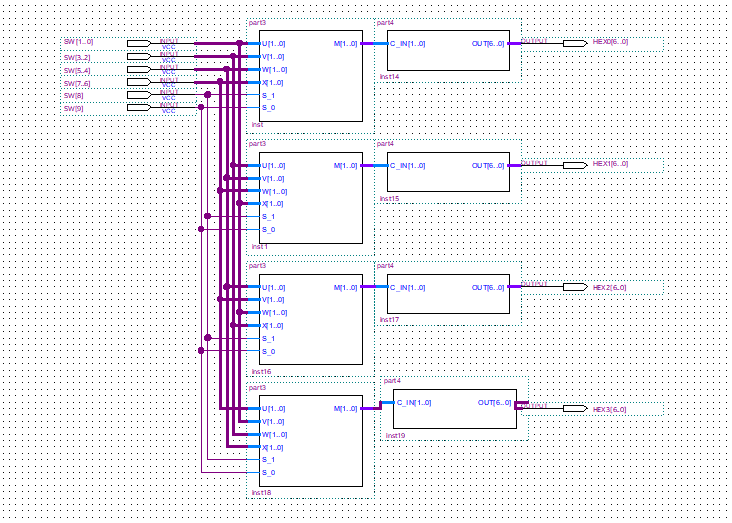
\includegraphics[width=\textwidth]{source/picture/Lab1/Lab1_5.png}
    \caption{Schematic for part 5}
\end{figure}
\clearpage

\section{Part VI }
\begin{itemize}
    \item [] \textbf{REQUIREMENT}
        \begin{enumerate}
            \item Extend your design from Part V so that is uses all 7-segment displays on your DE-series board. Your circuit needs to display a three- or four-letter word, corresponding to Table 2, using 'blank' characters for unused displays. Implement rotation of this word from right-to-left as indicated in Table 4 and Table 5. 
            \item Note that for the DE10-Lite you will need to use 3-bit codes for your characters, because five characters are needed when including the 'blank' character (your 7-segment decoder will have to use 3-bit codes, and you will need to use 3-bit wide 6-to-1 multiplexers). 
        \end{enumerate}
    \item [] \textbf{SOLUTION}
        \begin{lstlisting}[language=Verilog]
module part6(SW,HEX0, HEX1, HEX2, HEX3, HEX4, HEX5, HEX6, HEX7);
	input 	[2:0]SW;
	output 	[6:0]HEX0,HEX1,HEX2, HEX3, HEX4, HEX5, HEX6, HEX7;
	wire		[55:0]hex0,hex1,hex2,hex3,hex4,hex5,hex6,hex7;
	wire		[55:0]temp;

	assign hex0 = {7'b1111111,7'b1111111,7'b1111111,7'b1111111,7'b0100001,7'b0000110,7'b1111001,7'b1111111};
	assign hex1 = {7'b1111111,7'b1111111,7'b1111111,7'b0100001,7'b0000110,7'b1111001,7'b1111111,7'b1111111};
	assign hex2 = {7'b1111111,7'b1111111,7'b0100001,7'b0000110,7'b1111001,7'b1111111,7'b1111111,7'b1111111};
	assign hex3 = {7'b1111111,7'b0100001,7'b0000110,7'b1111001,7'b1111111,7'b1111111,7'b1111111,7'b1111111};
	assign hex4 = {7'b0100001,7'b0000110,7'b1111001,7'b1111111,7'b1111111,7'b1111111,7'b1111111,7'b1111111};
	assign hex5 = {7'b0000110,7'b1111001,7'b1111111,7'b1111111,7'b1111111,7'b1111111,7'b1111111,7'b0100001};
	assign hex6 = {7'b1111001,7'b1111111,7'b1111111,7'b1111111,7'b1111111,7'b1111111,7'b0100001,7'b0000110};
	assign hex7 = {7'b1111111,7'b1111111,7'b1111111,7'b1111111,7'b1111111,7'b0100001,7'b0000110,7'b1111001};
	
	assign temp = (SW==0)?hex0: 
					  (SW==1)?hex1:
					  (SW==2)?hex2:
					  (SW==3)?hex3:
					  (SW==4)?hex4:
					  (SW==5)?hex5:
					  (SW==6)?hex6:hex7;
					  
	assign HEX0 = temp[6:0];
	assign HEX1 = temp[13:7];
	assign HEX2 = temp[20:14];
	assign HEX3 = temp[27:21];
	assign HEX4 = temp[34:28];
	assign HEX5 = temp[41:35];
	assign HEX6 = temp[48:42];
	assign HEX7 = temp[55:49];
	
endmodule
    \end{lstlisting}
\end{itemize}

\clearpage



\begin{figure}[h]
    \centering
    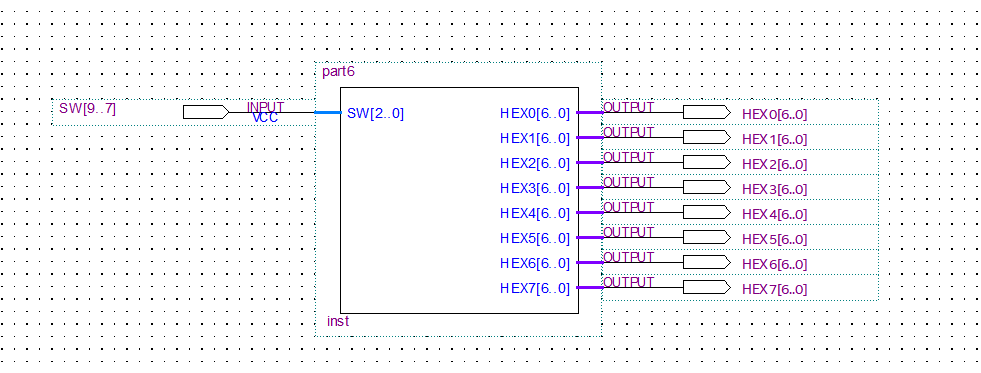
\includegraphics[width = \textwidth]{source/picture/Lab1/Lab1_6.png}
    \caption{Schematic for part 6}
\end{figure}

\begin{figure}[h]
    \centering
    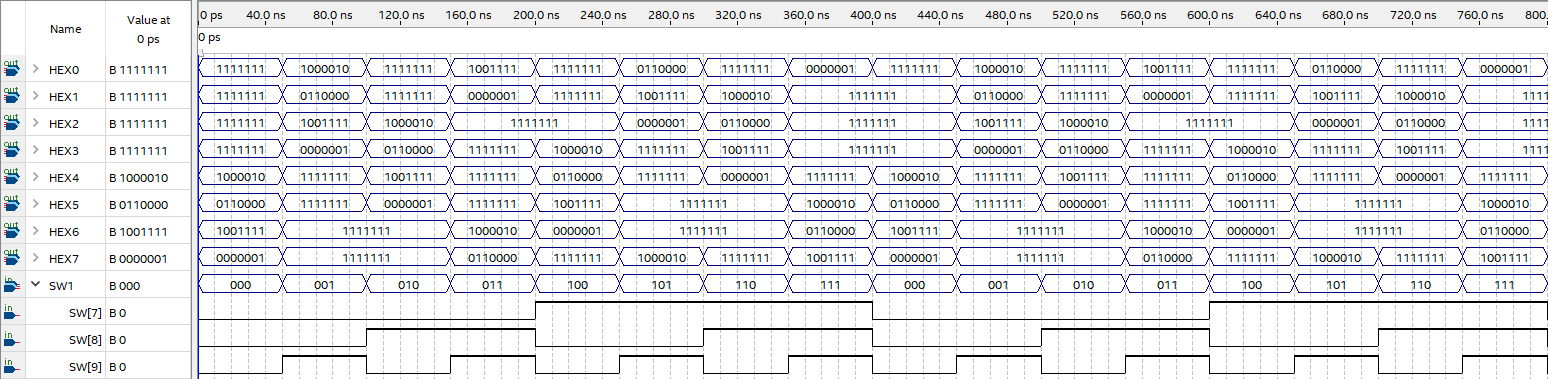
\includegraphics[scale = 0.40]{source/picture/Lab1/Lab1_wave.png}
    \caption{Simulation Result}
\end{figure}
\chapter{Background Theory}
\section{AMD Xilinx Kria KV260 platform}
\begin{center}
    \begin{figure}[H]
        \begin{center}
            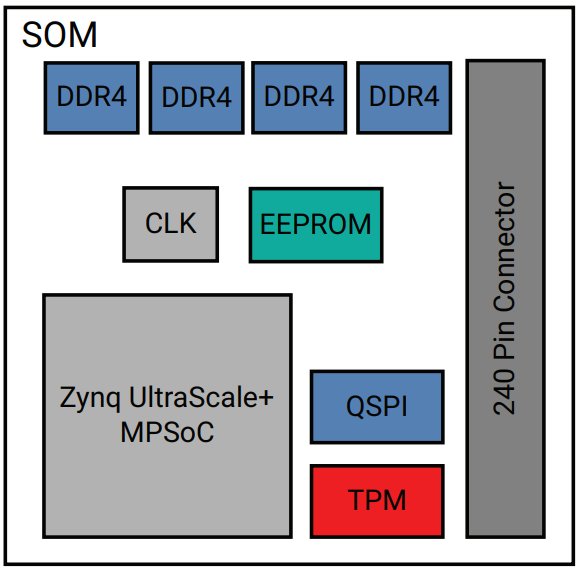
\includegraphics[width=5cm]{picture/kria/block_diagram.png}
        \end{center}
        \caption{K26 SOM Block Diagram}
        \label{ref Figure}
    \end{figure}
\end{center}
Kria KV260 is a board kit for developing AI vision applications. This
board kit has built-in hardware components supporting various applications such as smart city, machine vision, security cameras, etc. This board kit includes the following:

\begin{itemize}
\item K26 SoM
\item 8 interfaces support camera connectivity
\item MIPI sensor interfaces
\item ISP
\item HDMI, DisplayPort Outputs
\item 1Gb Ethernet
\item microSD card
\end{itemize}

The strength of this kit comes from the built-in K26 System-on-Module (SoM). This SoM consists of XCK26 SoC Zynq Ultrascale+ MPSoC, 4GB 64-bit DDR4, 16GB eMMC, Trusted Platform Module (TPM), 512Mb QSPI,... XCK26 is designed to fit in the acceleration of vision AI application.

Kria accelerated applications are intended to create robust application-specific FPGA hardware designs with a basic software application. In an accelerated application, the programmable logic portion of the SoC is pre-built for the user. No modification is required to use it, although it is certainly possible if desired.
\begin{table}[H]
    \centering
    \begin{tabular}{|l|c|}
        \hline
            \textbf{Kria Accelerated Application} & \textbf{Description}  \\
        \hline
        \hline
            Smart Camera & Supports Face Detection  \\
        \hline
            AI Box, ReID & Multi-Stream Face \& Pedestrian Detection \\
        \hline
            Distributed Smart Camera &  Multi-Stream Tracking \& Re-Identification\\
        \hline
            Machine Vision Camera & OpenCV-Based Defect Detection \\
        \hline
            NLP & Real-time Audio Keyword Spotting \& AI Fusion \\
        \hline
    \end{tabular}
    \caption{Accelerated Applications for Kria SOM}
\end{table}
\section{PYNQ Framework}

PYNQ is an open-source project from Xilinx that make it easy to use IPs and platform by accessing PL parts. This allow users utilize Xilinx platforms such as IO processing and video streaming,...easily. PYNQ supports Zynq, Zynq UntraScale+, Zynq RFSoC, Alveo accelerator boards, and AWS-F1.

Using Python language and libraries, PYNQ allows users to exploit the parallel processing strength of PL. PYNQ also contains several hardware libraries called overlays. These libraries can be used to configure programmable logic for accelerating software applications. In addition, PYNQ allows users to program in the Jupyter Notebook environment, which is friendly to users and help users program easily.
\begin{center}
    \begin{figure}[H]
        \begin{center}
            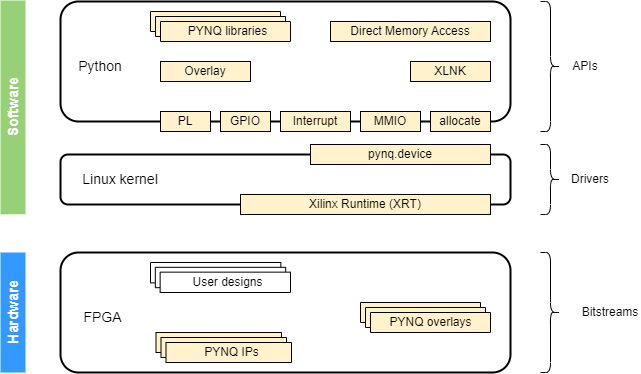
\includegraphics[width=9.5cm]{picture/pynq/pynq.drawio (1).png}
        \end{center}
        \caption{Overview about PYNQ Framework}
        \label{ref Figure}
    \end{figure}
\end{center}


\section{AXI (\textbf{A}dvanced e\textbf{X}tensible \textbf{I}nterface)}
AXI is an on-chip communication bus protocol developed by \href{https://en.wikipedia.org/wiki/Arm_(company)}{ARM} which is used in most Xilinx chips and many Xilinx IPs. Today, SoC contains many components in a single chip such as (Processors, UART, ADC/DAC, CPU, FPGA,...). AXI is designed for FPGAsbased on AMBA as a protocol for communication between blocks of IP. These are reasons for the must for AXI.

Here are some of the important features of an AXI interfaces:
\begin{itemize}
\item Support burst transactions with only start address issued
\item Different phases for the data and addresses
\item Write and Read channels are separated which causes the low-cost Direct Memory Access (DMA)
\end{itemize}

Regarding the nature of the design, there are two types of AXI4 interface which are shown in Fig. 2.3. 
\begin{itemize}
\item \textbf{AXI4:} Capable of doing memory map burst transaction up to 256 data transfer cycles per address phase.
\item \textbf{AXI4-Lite:} Utilized for the single bit memory map transaction.
\item \textbf{AXI-Stream:} There is no address channel and it allows an unlimited burst transaction between the master and slave.
\end{itemize}
\begin{center}
    \begin{figure}[H]
        \begin{center}
            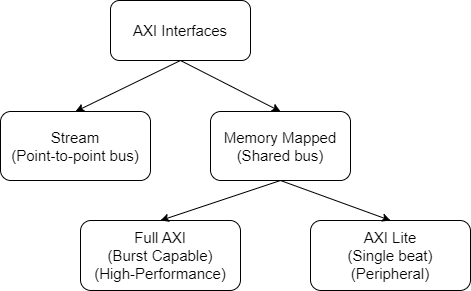
\includegraphics[width=8.5cm]{picture/AXI/axi2.drawio.png}
        \end{center}
        \caption{AXI interconnection flowchart}
        \label{ref Figure}
    \end{figure}
\end{center}

AXI communication happens between a Master and a Slave. Master component is the one to start the transaction of data. Xilinx has an AXI interconnection IP that allows communication between multiple Slaves and Masters. There is only connection between Master and Slave (there is no Master-Master or Slave-Slave connection).

There are 2 types of AXI: AXI Memory Map and AXI Stream. AXI Memory Map needs a destination address to transfer data. This type supports two ways of communication (Fig. 2.4). AXI Stream does not need a destination address because the communication is one-way (from a Master to a Slave)(Fig. 2.5). Therefore, it is a contiguous stream of data suitable for transferring large contiguous data such as video data from DRAM to PL.


\begin{center}
    \begin{figure}[H]
        \begin{center}
            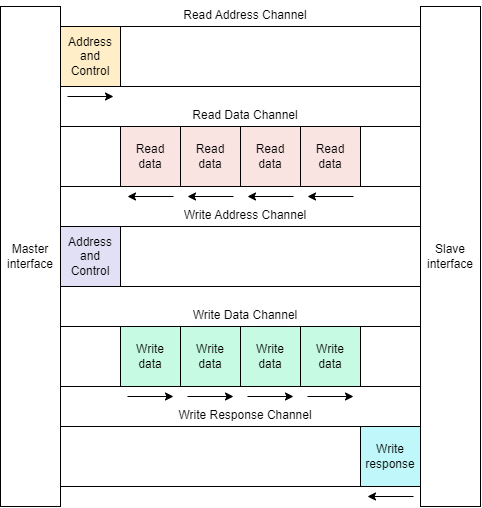
\includegraphics[width=7cm]{picture/AXI/AXI.drawio (1).png}
        \end{center}
        \caption{AXI Memory-mapped Interfaces}
        \label{ref Figure}
    \end{figure}
\end{center}
\begin{center}
    \begin{figure}[H]
        \begin{center}
            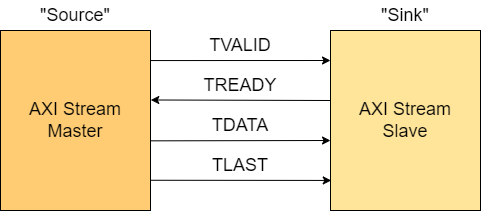
\includegraphics[width=7cm]{picture/AXI/AXI.drawio.png}
        \end{center}
        \caption{AXI Stream Interfaces}
        \label{ref Figure}
    \end{figure}
\end{center}

AXI connection is required for communication between PS and PL. Because Processor uses AXI3, AXI interconnection between PS and PL is used to convert AXI3 to AXI4 and AXI4-Lite (which is used by most of Xilinx IP) (Fig. 2.6). Every IP which has AXI memory map interface has address space. Base address and its range are generated automatically by Vivado. These parameters can edited due to users' demands. However, consider that address space of one component cannot overlap with others. The base address of a component is divisible by the space range. The space range must be large enough to be able to access all IP registers.

\begin{center}
    \begin{figure}[H]
        \begin{center}
            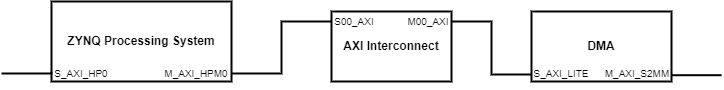
\includegraphics[width=14cm]{picture/AXI/pspl.drawio.png}
        \end{center}
        \caption{AXI Connection between PS and PL}
        \label{ref Figure}
    \end{figure}
\end{center}
\section{Decision Tree and Random Forest}
\subsection{Decision Tree}
Decision Tree is the algorithm belongs to the family of supervised learning algorithm. DT algorithm, in contrast to other supervised learning methods, is capable of handling both \textbf{classification and regression problems}.

In DTs, we begin at the tree's \textbf{root} when anticipating a record's class label. We contrast the root attribute's values with that of the attribute on the record and follow the branch corresponding to that value and move to the next node based on the comparison.

A DT has two types of nodes which are internal nodes and leaf nodes.
\begin{itemize}
\item An \textbf{internal node} has two child nodes. To determine which branch (left child or right child) will be chosen next, each internal node carries out a test on an attribute of a sample. A test, also referred to as a decision rule, compares an attribute with a threshold value. Thresholds can be obtained during the DT training process.
\item A \textbf{leaf node} has no child node. Each leaf node contains a prediction value, a class label for classification, or a numeric value for regression. A prediction of a single DT will end if a leaf node is encountered.
\end{itemize}
For predicting, an input is first fed to the root node. The sample travels down the tree through each terminal node until it reaches a leaf node. Figure 2.7 shows an example of a decision tree.
\begin{center}
    \begin{figure}[H]
        \begin{center}
            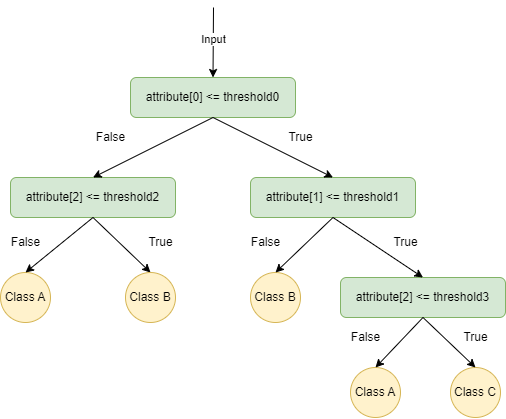
\includegraphics[width=11cm]{picture/algo/decisiontree.drawio.png}
        \end{center}
        \caption{A single simple decision tree}
        \label{ref Figure}
    \end{figure}
\end{center}
There are some advantages DT has as follows:
\begin{itemize}
    \item DT is simple to understand, interpret and visualize.
    \item DT can be used to predict both continuous and discrete values.
    \item DT can handle multiple types of data whether it is numerical, categorical or boolean.
    \item Training and predicting data does not require much pre-processing as other
machine learning algorithms.
    \item Don't need to worry about feature scaling.
    \item DT does not require any transformation of the features when dealing with non-linear data.
\end{itemize}
However, this such algorithm also meets some drawbacks:
\begin{itemize}
    \item Prediction of DT is easy to be overfitting. To solve the problem, setting constraints on the parameters model and pruning method need to be done.
    \item A small change in the data can cause a large change in the structure of DT causing instability.
    \item DT can be highly time-consuming in its training phase, and this problem can be exaggerated if there are multiple continuous independent variables.
    \item It is difficult for DT to interpret complex logic such as multiplexer or XOR.
   \item After training, DT can encounter high bias if some classes make up the majority.
\end{itemize}
As mentioned above, the common problem of DT is overfitting. This affects the accuracy when predicting samples that are not part of the training set. Therefore, there are 2 ways to remove overfitting which is using \textbf{Prunning method} and \textbf{Random Forest}. We will discuss about \textbf{Random Forest} in the next section.
\\

\textsc{\textbf{Pruning}}

\textbf{Pruning} is a technique that removes the branches of DT which prevent it from growing to its full depth. These branches eliminated from the tree are the parts that  have less contribution to classify instances. There are two types of pruning: \textbf{Pre-pruning} and \textbf{Post-pruning}.

\textbf{Pre-pruning} slows the growth of the decision tree and prevents it from reaching its maximum depth. Early stopping is to avoid manufacturing leaves with small samples. Some hyperparameters  can be tuned for early stopping and preventing overfitting such as maximum depth of DT, minimum number of samples on each leaf, and minimum number of samples required to split an internal node. However, DT can be underfitting if hyperparameters are chosen irregularly.

\textbf{Post-pruning} cuts back branches of a DT after it is completely grown. Subtrees are iteratively created until there is an optimal subtree with the highest cross-validation. A subtree, in this case, is a subtree that has the same root as the original tree. One technique for post-pruning is Cost Complexity Pruning, also known as Weakest Link Pruning score. This technique calculates the cost complexity based on Sum of Squared Residuals (SSR) and Penalty on the Complexity ($\alpha |T|$) as shown in the equations below (Equation 2.1 and 2.2). 
\begin{align}
C_\alpha(T) = SSR + \alpha |T|\\
SSR = \sum_{i=1}^n (y_{train_i} - y_{test_i})^2
\end{align}

where:

$T$ is the total number of leaves

$\alpha$ is a complexity parameter that controls the number of leaf nodes

$y_{train_i}$ is the training data samples

$y_{test_i}$ is the testing data samples\\

Training data is used to prune the tree based on $\alpha$ value. Testing data is used to calculate tree scores of previously pruned subtrees. The subtree with the minimum $C_\alpha(T)$ will be selected as the resulting subtree.

In order to get Weakest Link Pruning score, we need to choose the optimal $\alpha$ due to using \textbf{Cross-Validation}. This is the parameter that minimizes the validation error and avoid Overfitting.

\subsection{Random Forest}
Random Forest (RF) is an ensemble learning algorithm for solving classification and
regression problems and was first introduced by Ho in \cite{aHo}. A single forest consists of many decision trees that contribute to the prediction’s final result and are trained with bootstrap aggregating (bagging) algorithm \cite{breiman}. The prediction result of RF is created by taking the mean or average (regression) or majority (classification) of results derived from individual DTs. Figure 2.8 describes a general architecture of RF. 

In comparison with DT, RF has some important key benefits\autocite{cRF}:
\begin{itemize}
\item \textbf{Reduce risk of overfitting:} DTs run the risk of overfitting as they tend to tightly fit all the samples within training data. However, when there’s a robust number of DTs in a RF, the classifier cannot overfit the model since the averaging of uncorrelated trees lowers the overall variance and prediction error.
\item \textbf{Provide flexibility:} RF can handle both regression and classification tasks with a high degree of accuracy. The RF classifier is a useful tool for guessing missing values due to feature bagging since it retains accuracy even when some of the data is missing.
\item \textbf{Easy to determine feature importance:} To attain similar precision in DT, a user has to choose the hyperparameter for tuning carefully. Specificially, Gini importance and mean decrease in impurity (MDI) are usually used to measure how much the model’s accuracy decreases when a given variable is excluded
\end{itemize}

 However, one of the most significant disadvantages of RF is that it has a large number of trees in order to have high accuracy. This can make the algorithm predicts slowly and is hard to meet the real-time requirement. In addition, RF has low performance working with spatially non-stationary data, as shown in the research of Hui Wan.

\begin{center}
    \begin{figure}[H]
        \begin{center}
            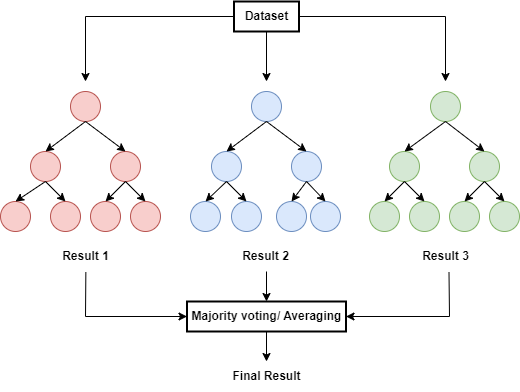
\includegraphics[width=10cm]{picture/algo/rf.drawio.png}
        \end{center}
        \caption{A simple example of random forest}
        \label{ref Figure}
    \end{figure}
\end{center}

\textsc{\textbf{Bagging}}\cite{dkdN}

Bagging stands for Bootstrap Aggregating. As
the name suggests, this algorithm consists of two phases: bootstrapping and aggregating. This method comes from the "wisdom of crowds," meaning that many decision-makers are more significant than any individual decision-maker.

\textbf{Bootstrapping} is a technique used for training a ML model. DTs are very sensitive to the data they are trained on, small changes to the training data set can result in a significantly different tree structure. In contrast, RF takes advantage of this by allowing each individual tree to randomly sample from the dataset with replacement, resulting in different trees which are called bootstrapped datasets.

\textbf{Aggregation} is collecting results from different DTs to makeout a final prediction. If it is a classification problem, a majority voting will be used to decide the final result. Otherwise, averaging will be used to solve the regression problem.\\

\textsc{\textbf{Hyperparameter}}\cite{eupgrad}

There are various hyperparameters that can be controlled in a RF. However, in Scikit-learn package library, there is an automatic tuning can be obtained by the grid-search method, which finds optimal hyperparameters through specifying feature importance
\begin{itemize}
\item \textbf{n\_estimators:} The number of DTs being built in the forest. These are the most important hyperparameters that the user has to investigate first.
\item \textbf{max\_depth:} The maximum levels allowed in a DT.
\item \textbf{max\_features:} The maximum number of features considered when splitting a node.
\item \textbf{min\_samples\_split:} The minimum number of samples required to split an internal node.
\item \textbf{min\_samples\_leaf:} The minimum number of data point requirements in a node of the DT.
\item \textbf{max\_leaf\_nodes:} The condition can be set on the splitting of the nodes in the tree in order to restrict the growth of the tree
\item \textbf{bootstrap:} The type of value is boolean. True means sampling data with bootstrap. False means sampling data without bootstrap.
\end{itemize}
\section{Clock Domain Crossing}
\subsection{Basic knowledge} \cite{anysilicon}
Clock Domain Crossing (CDC) is defined as: "The process of passing a signal or vector (multi bit signal) from one clock domain to another clock domain.”. Two clock domains are considered to be asynchronous when they use two unrelated clocks (different clock frequencies) or clocks from two different sources (even with same frequency). 

\begin{center}
    \begin{figure}[H]
        \begin{center}
            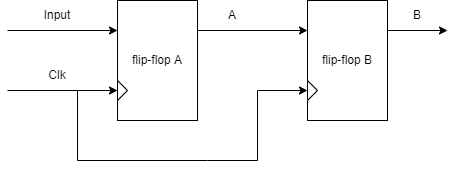
\includegraphics[width=9cm]{picture/CDC/hinh 1.png}
        \end{center}
        \caption{Single Clock domain}
        \label{ref Figure}
    \end{figure}
    
    \begin{figure}[H]
        \begin{center}
            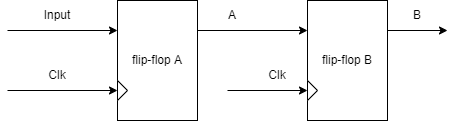
\includegraphics[width=10cm]{picture/CDC/hinh 2.png}
        \end{center}
        \caption{Multiple Clock domains}
        \label{ref Figure}
    \end{figure}
\end{center}

\subsection{Metastability}  \cite{anysilicon}
“Metastability” is referred as unstable state. When a signal enters metastability, it might not have reached to expected value and can oscillate between 0 or 1. Metastability may cause a fatal system failure in critical timing design projects. Avoidance of matastability in digital design when transferring data between 2 different clock domains is impossible but can be handled properly by using different CDC techniques.

Metastability appears since the appearance of "setup time" ($t_{su}$) and "hold time" ($t_{h}$). Setup Time is when input data signals are stable (either high or low) before the active clock edge occurs. Hold Time is when input data signals are stable (either high or low) after the active clock edge occurs.

Metastability occurrence of flip-flop can be predicted by using a parameter called MTBF. MTBF can be caculated when knowing input rate and the clock frequency.
\begin{center}
    \begin{figure}[H]
        \begin{center}
            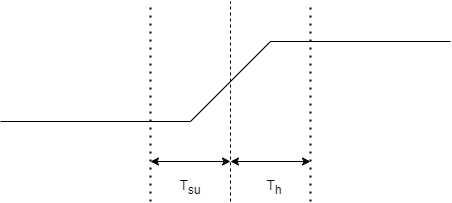
\includegraphics[width=7cm]{picture/CDC/setup-hold time.png}
        \end{center}
        \caption{Setup time and Hold time}
        \label{ref Figure}
    \end{figure}
    \begin{figure}[H]
        \begin{center}
            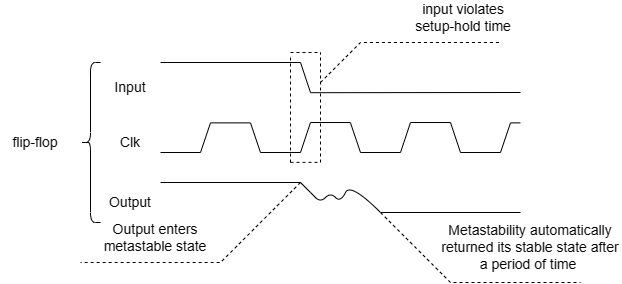
\includegraphics[width=11cm]{picture/CDC/metastability.png}
        \end{center}
        \caption{Setup - Hold time violation causes metastability}
        \label{ref Figure}
    \end{figure}
\end{center}



\subsection{Clock Multiplexer (Clock MUX)}
Clock MUX is used to operate the same logic function with different clock sources. With Clock MUX, we can switch the source of a clock line while the chip is running and the MUX will be controlled by one or some internal logic.

Clock MUX has many inputs and a control signal to choose which input is propagated to output. However, implementing clock MUX by a normal MUX is impossible since Glitches and timing problems (metastability, data missing,...).

A glitch may be caused due to immediate switch of output from Current Clock source to Next Clock source, when the Select value changes. The problem with this switch is the switch control signal can change any time, thus creating a potential for chopping the output clock or creating a glitch at the output.

\begin{center} 
    \begin{figure}[H]
        \begin{center}
            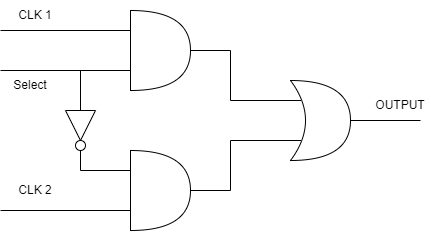
\includegraphics[width=7cm]{picture/clock mux/clock mux-Page-2.drawio.png}
        \end{center}
        \caption{Clock MUX using normal MUX}
        \label{ref Figure}
    \end{figure}
\end{center}

\begin{center} 
    \begin{figure}[H]
        \begin{center}
            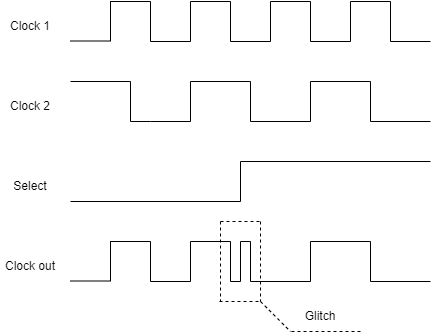
\includegraphics[width=8cm]{picture/clock mux/clock mux.drawio.png}
        \end{center}
        \caption{How a glitch is generated}
        \label{ref Figure}
    \end{figure}
\end{center}

A solution to prevent glitch at the output is using D flip-flop. Negative edge triggered D-ff is inserted in the selection path for each of the clock sources. By this technique, clocks are be stored in flip-flops and released when flip-flop active. When the select signal changes, output will not change immediately, but waits until the clock actives low and starts the propagation at the next negative edge of the new clock.
\begin{center} 
    \begin{figure}[H]
        \begin{center}
            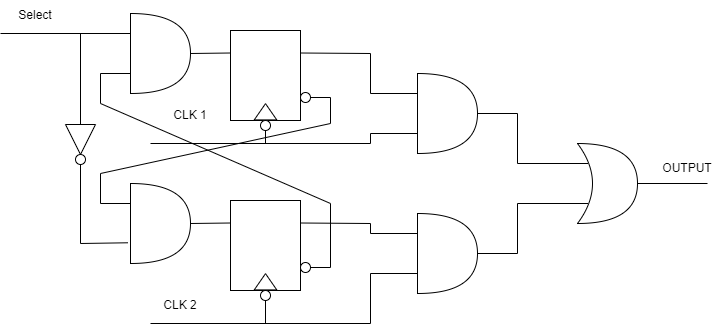
\includegraphics[width=10cm]{picture/clock mux/clock mux-Page-3.drawio.png}
        \end{center}
        \caption{Clock MUX adding D flip-flop}
        \label{ref Figure}
    \end{figure}
\end{center}

\begin{center} 
    \begin{figure}[H]
        \begin{center}
            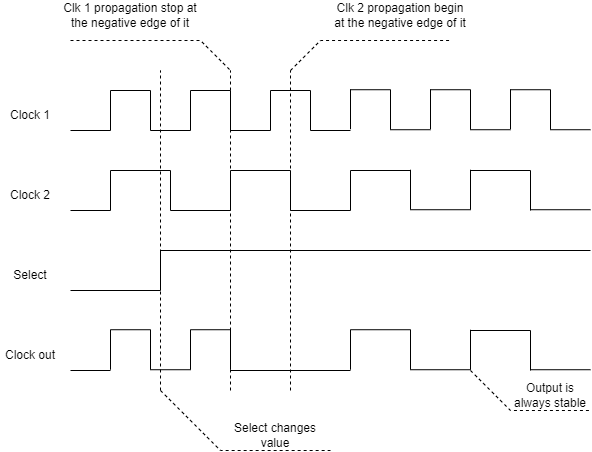
\includegraphics[width=10cm]{picture/clock mux/clock mux-Page-4.drawio.png}
        \end{center}
        \caption{How a glitch is freed}
        \label{ref Figure}
    \end{figure}
\end{center}

\chapter{Implementation}
Now comes the essential part of the report. We spend the first sub-section describes about FIFO and BRAM are the main channels to transfer data. Then we will go through some computing IP catalogs. After that, data flow of convolution computing core and implementation of some essential modules and interconnecting communication that exist among the data flow. 
\section{FIFO}

\cite{nandland}FIFO stands for First in First out. FIFO is the buffer which is used for storing and transferring data with the structure: the data written into the buffer first comes out of it first.

FIFO is the special memory since instead of reading/writing from any location with specific address like RAM, FIFO stores data by arranging from one address and address pointer kept on incrementing. The order (before - after) of data is the key issue of FIFO.

In FPGA and ASIC design, FIFO is popular for any below purposes:
\begin{itemize}
    \item It is necessary to store a relatively amount of data, compared with single registers. The size of these data amount is usually not too large.
    \item It is necessary to temporarily store a certain amount of data for synchronizing between 2 clock  domains with different pulses.
    \item It is necessary to store an amount of data which is the unit of computing process.
\end{itemize}

\subsection{The principle of operation}
FIFO is designed for different purposes but in basic, it has to follow 2 flags called: "empty" and "full"; and the 2 "most basic" principles is:
\begin{itemize}
    \item Never write into a full FIFO (FIFO at "full" state) since resulting in memory leakage.
    \item Never read from an empty FIFO (FIFO at "empty" state) since reading unexpected signal.
\end{itemize}

The most vital thing when using FIFO is calculating its depth. It is necessary to assure FIFO design is compatible for 2 requirements: no memory leak and right amount of memory using.

\subsection{FIFO Design}
FIFO is also designed in different ways. The most general diagram of FIFO is using synchronous RAM block with 2 independent read and write ports. After reading data, it is considered to be excluded from the buffer, leave space for other data to be written.
\begin{figure}[H]
    \centering
    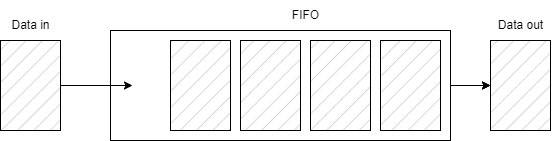
\includegraphics[width = 8cm]{picture/fifo/fifo.drawio.png}
    \caption{FIFO structure}
    \medskip
\end{figure}
As mentioned above, the phenomenon of address in FIFO is ignored. There are 2 pointers, one used for reading (Read pointer), the other used for writing (Write pointer). Assume that memory parts are located inside a circle with 2 pointers (Read pointer and Write pointer). First, Read pointer and Write pointer are at the initial state. Then, increment Read pointer to write data into the buffer. After write some data, increase Write pointer to read data. The process is repeated.
\begin{figure}[H]
    \centering
    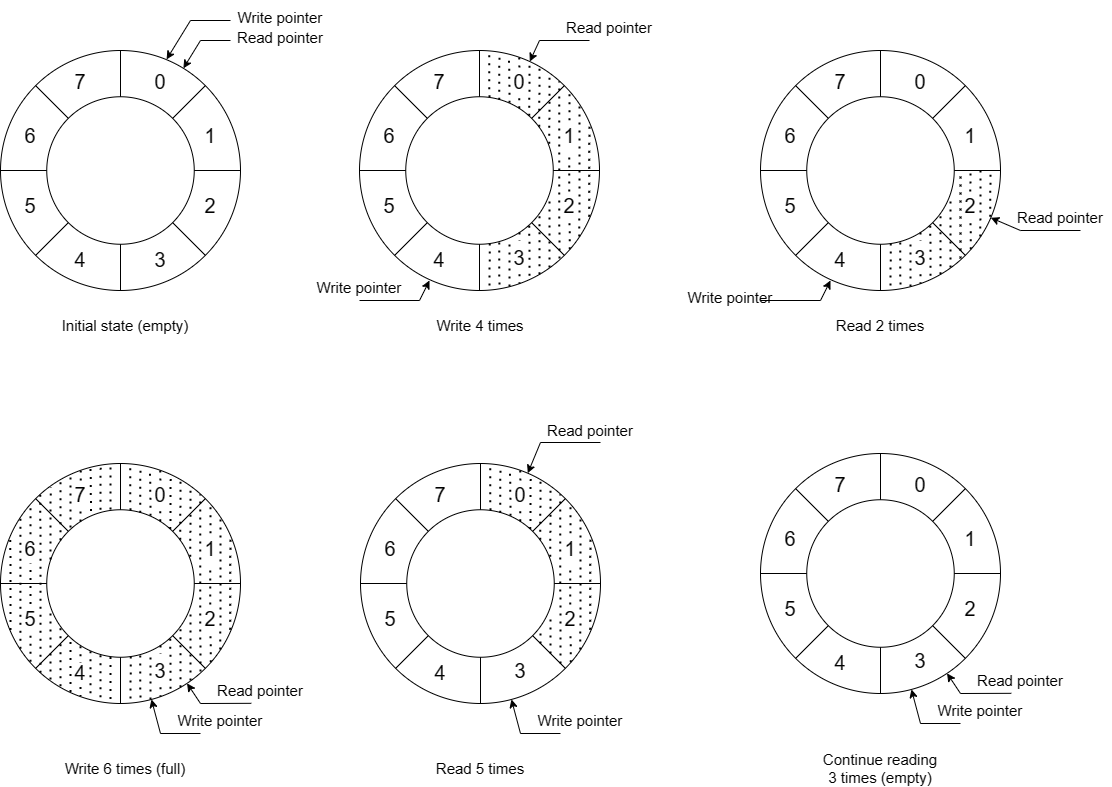
\includegraphics[width = 11cm]{picture/fifo/fifo-image.drawio.png}
    \caption{FIFO operation}
    \medskip
\end{figure}

From the example, it is realized that the FIFO not only uses 2 pointers (Read pointer and Write pointer) but also needs 2 flags: empty and full
\begin{itemize}
    \item Flag empty is used to determine the empty state of FIFO. This flag avoids from reading empty data.
    \item Flag full is used to determine the full state of FIFO. This flag avoids from overwritten data (or leaking memory)
\end{itemize}
\section{BRAM (Buffer Random Memory Access)}
\subsection{Memory Type}
Block Memory Generator core is a tool allows users to create various types of memory blocks  in DCs. These memory types include Single-port RAM, Simple Dual-port RAM, True Dual-port RAM, Single-port ROM, and Dual-port ROM. \textbf{Simple Dual-port RAM} configuration is chosen as example as follows.
\begin{figure}[H]
    \centering
    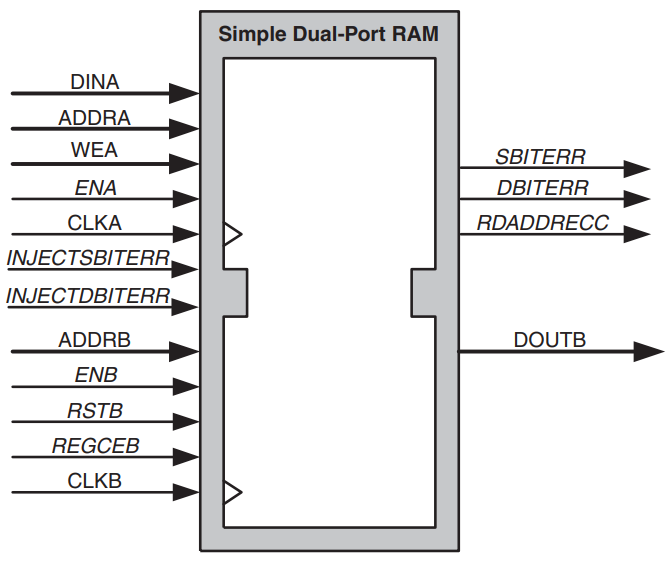
\includegraphics[width = 6.5cm]{picture/BRAM/dual-port.png}
    \caption{Simple Dual-port RAM}
    \medskip
\end{figure}
Simple Dual-port RAM is a type of memory that has 2 separate ports (A and B). Port A is used for write access to the memory and Port B is used for read access to the memory. This type of memory is useful when multiple parties need to access the memory simultaneously. However, using the Simple Dual-port RAM can result in conflicting updates to the data stored in that location.
\subsection{Synchronous Write-Read Collisions}
Synchronous Write-Read collision might occur if a port attempts to Write a memory location and the other port reads the same location. While memory contents are not corrupted in Write-Read collisions, the validation of the output data depends on the Write port operating mode.
\begin{itemize}
    \item If Write port is in READ\_FIRST mode, Read port can rely on the old data of the memory location because Write port reads the old contents of the memory location then stores them temporarily, and writes new data to the same location.
    \item If Write port is in WRITE\_FIRST or NO\_CHANGE mode, the output of the Read port is invalid. In WRITE\_FIRST mode, Write port writes new data to memory location before Read port has a chance to read the old data. In NO\_CHANGE mode, Write port does not update the data in the memory location, so the Read port will output the same data as before.
    \item In case of byte-writes, where only certain bytes of the memory location are updated, the output of the Read port will be invalid only for the updated bytes. It is important to consider these Write-Read collision scenarios when using the Simple Dual-port RAM in a digital circuit to ensure the correctness of the data output by the Read port.
\end{itemize}
\subsection{Selectable Memory Algorithm}
BMG core contains 1 to 4608 bits width. The maximum depth of the memory is limited only by the number of block RAM primitives in the target device. The core configures block RAM primitives and connects them together using one of the following algorithms:
\begin{itemize}
    \item \textbf{Minimum Area Algorithm}: Generate the memory using the minimum number of block RAM primitives, while still allowing for the use of both data and parity bits. 
    \item \textbf{Low Power Algorithm}: Minimize the number of block RAM primitives that are enabled during a Read or Write operation. This can result in a lower power consumption for the memory.
    \item \textbf{Fixed Primitive Algorithm}: Generate the memory using only a single type of block RAM primitive. This can be useful in situations where a specific type of primitive is preferred or required. 
\end{itemize}

\section{Computing IP Catalog}
\subsection{Adder/Subtracter IP}
The adder/subtracter ip can generate adders (a+b), subtracter (a-b) and
dynamically configurable adder/subtracters that operate on signed or unsigned data.
\begin{figure}[H]
    \centering
    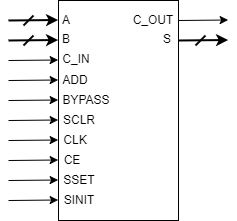
\includegraphics[width = 5.5cm]{picture/IP Catalog/add/Core_symbol.png}
    \caption{Adder/Subtracter IP Core Symbol}
    \medskip
\end{figure}

Adder/Subtracter module can be optionally pipelined to improve speed. The pipelined operation is controlled by the latency parameters. When set it to manual, module allows a valid number of pipeline stages to be entered in the Latency parameter.

\begin{figure}[H]
    \centering
    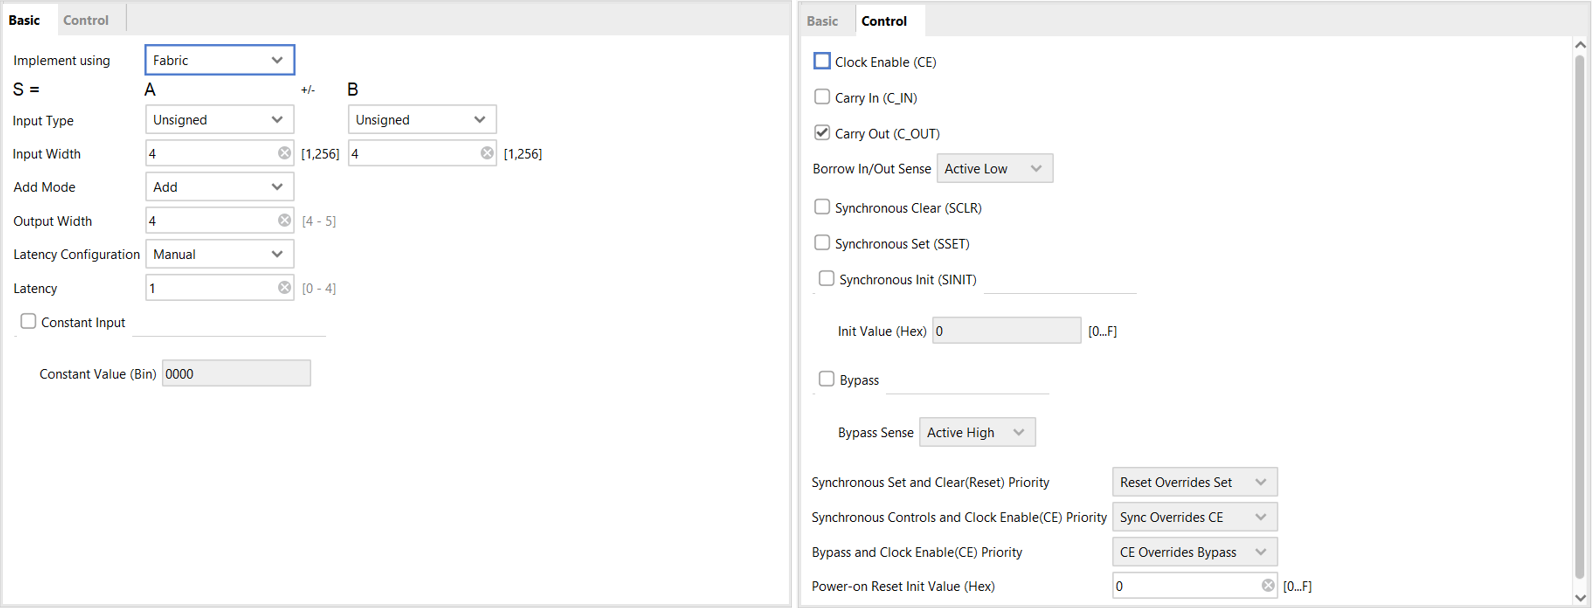
\includegraphics[width = 15cm]{picture/IP Catalog/add/ipaddcustom.png}
    \caption{Adder/Subtracter IP customization}
    \medskip
\end{figure}

\subsection{Multiplier IP}
IP Multiplier implements high-performance, optimized multipliers. A number of resource and performance trade-off options are available to tailor the core to a particular application. It also can generate dynamically configurable Multipliers that operate on signed/unsigned data.

\begin{figure}[H]
    \centering
    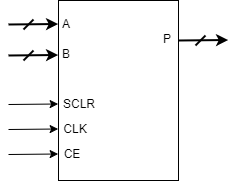
\includegraphics[width = 6cm]{picture/IP Catalog/mul/Core_symbol_mul.png}
    \caption{Multiplier IP Core Symbol}
    \medskip
\end{figure}

\begin{table}[H]
    \centering
    \begin{tabular}{|l|c|l|}
        \hline
            \textbf{Name} & \textbf{Direction} & \textbf{Description}  \\
        \hline
        \hline
            A[N-1:0] & Input & A operand input bus, N bits wide \\
        \hline
            B[M-1:0] & Input & B operand input bus, M bits wide (parallel multipliers only) \\
        \hline
            CLK & Input & Clock signal: rising edge \\
        \hline
            CE & Input & Active high Clock Enable \\
        \hline     
            SCLR & Input & Active high Synchronous Clear (SCLR/CE priority is configurable) \\
        \hline
            P[X:Y] & Output & Product Output – bit X down to bit Y \\
        \hline
    \end{tabular}
    \caption{Multiplier IP Core Signal Pinout}
\end{table}

\begin{figure}[H]
    \centering
    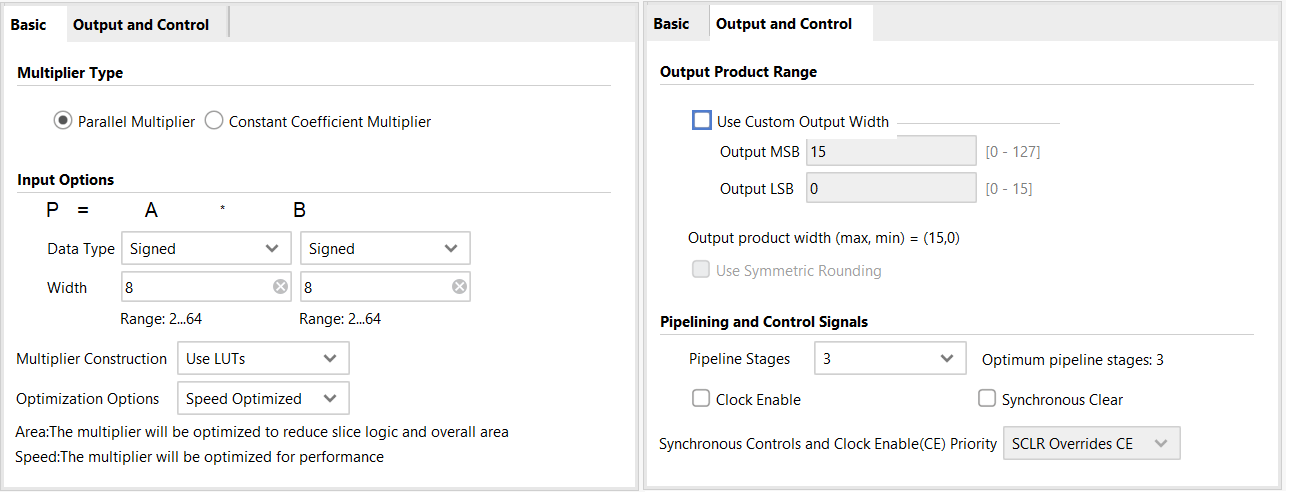
\includegraphics[width = 14cm]{picture/IP Catalog/mul/ipmulcustom1.png}
    \caption{Multiplier IP customization}
    \medskip
\end{figure}

\subsection{Floating-point IP}

The floating-point ip compliance with IEEE-754 Standard and supports many operators: multiply, add/subtract, divide, comparison, conversion from floating-point to fixed-point, fixed-point to floating-point, and between floating-point types,...

The ip supports a different range of fraction and exponent wordlength with basic formats:
\begin{itemize}
    \item \textbf{Binary 16 bits (Half Precision Format:)} Uses 16 bits, with an 11-bit fraction and 5-bit exponent.
    \item \textbf{Binary 32 bits (Single Precision Format):} Uses 32 bits, with a 24-bit fraction and 8-bit exponent. 
    \item \textbf{Binary 64 bits (Double Precision Format):} Uses 64 bits, with a 53-bit fraction and 11-bit exponent. 
    \item \textbf{Binary 128 bits (Quadruple Format):} not supported
\end{itemize}
\subsubsection{Port Descriptions}
\begin{figure}[H]
    \centering
    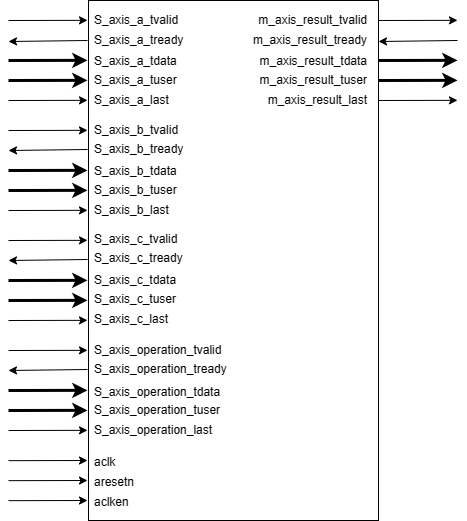
\includegraphics[width = 8cm]{picture/IP Catalog/floating/ip-Page-1.drawio.png}
    \caption{Floating-point IP Core Symbol}
    \medskip
\end{figure}

\subsubsection{Non-Blocking Mode}
The term Non-Blocking means that lack of data on one input channel does not block the execution of an operation if data is received on another input channel. Without the facility to block dataflow, the internal implementation is much simplified, so fewer resources are required for this mode.

Operations occur on every enabled clock cycle and data is presented on the output regardless of TVALID. But when all of the input channels receive an active TVALID, an operation is validated and the output TVALID (suitably delayed by the latency of the core) sends an active signal to inform when the operation done. 

\begin{figure}[H]
    \centering
    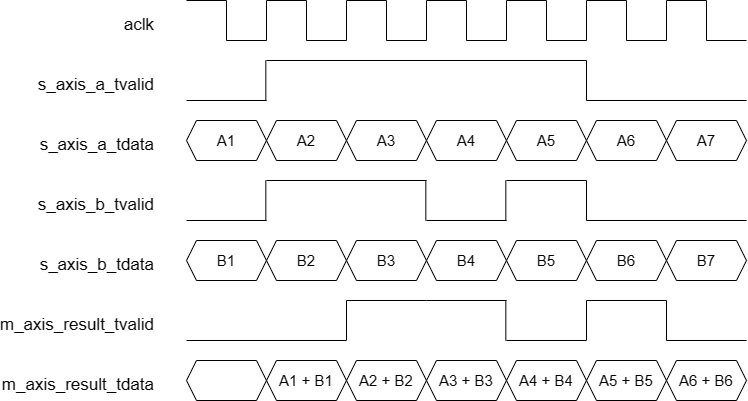
\includegraphics[width = 10cm]{picture/IP Catalog/floating/ip-Page-2.drawio.png}
    \caption{Non-Blocking Mode}
    \medskip
\end{figure}

\subsubsection{Blocking Mode}
The term Blocking means that operation execution does not occur until fresh data is available on all input channels. This mode prevents data loss with the control of TREADY. When all input channels have validated data available, an operation occurs and the result becomes available on the output. If TREADY is low then data accumulates in the output buffer internal to the core. When this output buffer is nearly full the core stops further operations.

This mode is also required that before each operation, all the inputs must receive validated data. Therefore when at least one input channel does not receive validated data while others do, the validated data is stored in the input buffer of the channel. And after some cycles of data storage, the first data on channel A is paired with the first data on channel B, the second with the second and so on

\begin{figure}[H]
    \centering
    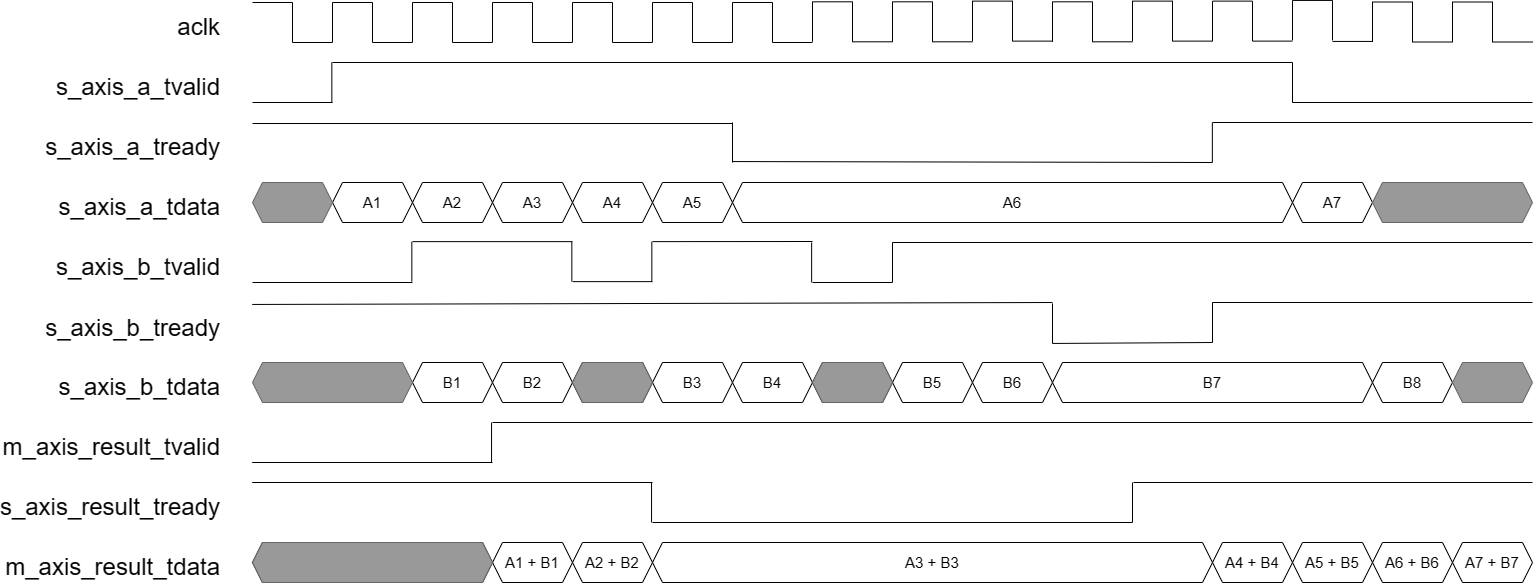
\includegraphics[width = 15cm]{picture/IP Catalog/floating/ip-Page-21.drawio.png}
    \caption{Blocking Mode}
    \medskip
\end{figure}
\subsubsection{IP customization}
\begin{figure}[H]
    \centering
    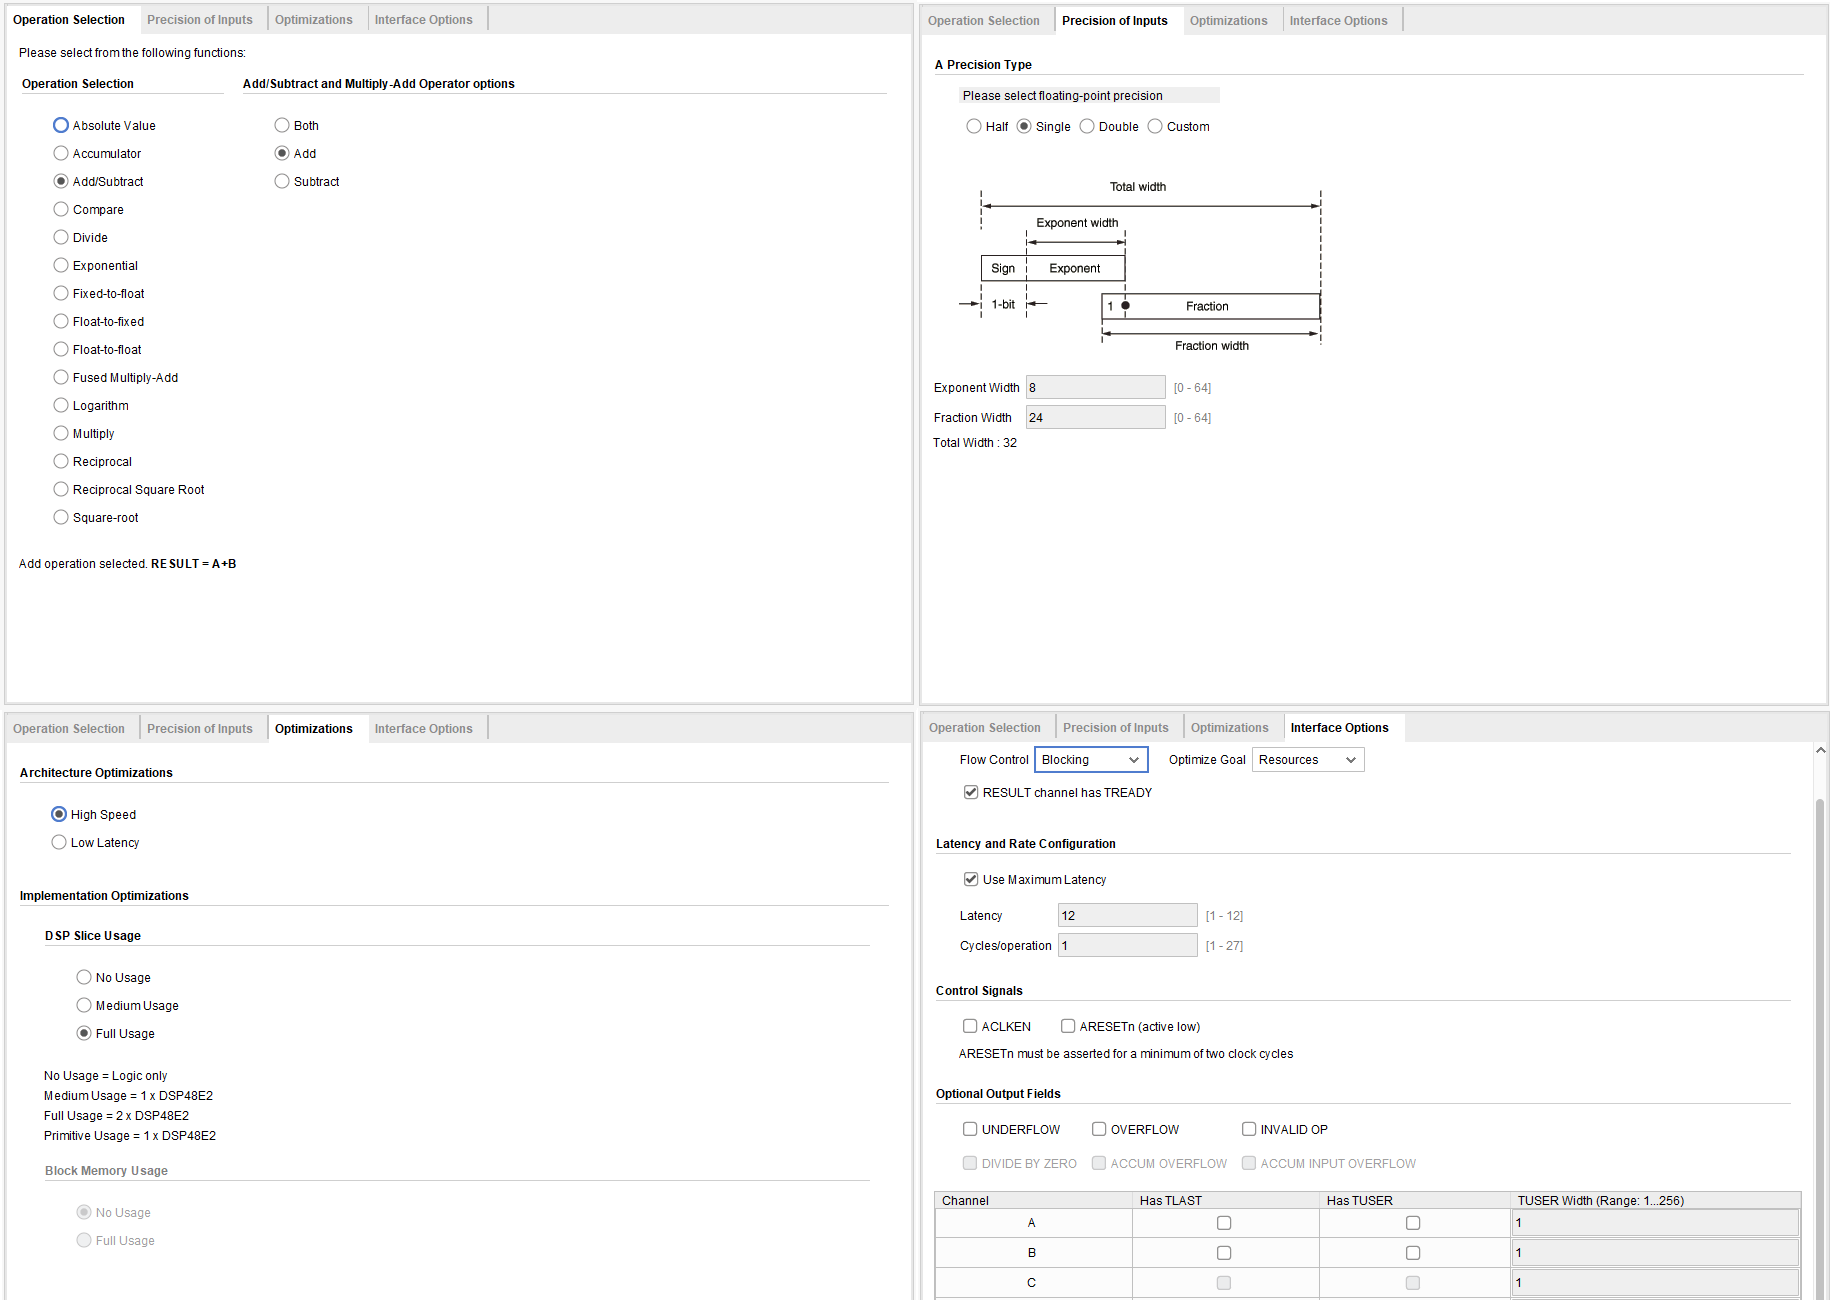
\includegraphics[width = 15cm]{picture/IP Catalog/floating/ipfloatcustom.png}
    \caption{Floating-point IP customization}
    \medskip
\end{figure}

\section{PS - PL Communication}
\subsection{PYNQ AXI DMA to FIFO}
DMA allows users to stream data from memory, PS DRAM in this case, to an AXI stream interface. This is called the READ channel of the DMA. The DMA can also receive data from an AXI stream and write it back to PS DRAM. This is the WRITE channel.

DMA has AXI Master ports for the read channel, and another for the write channel, and are also referred to as memory-mapped ports - they can access the PS memory. The ports are labelled MM2S (Memory-Mapped to Stream) and S2MM (Stream to Memory-Mapped). 
\begin{figure}[H]
    \centering
    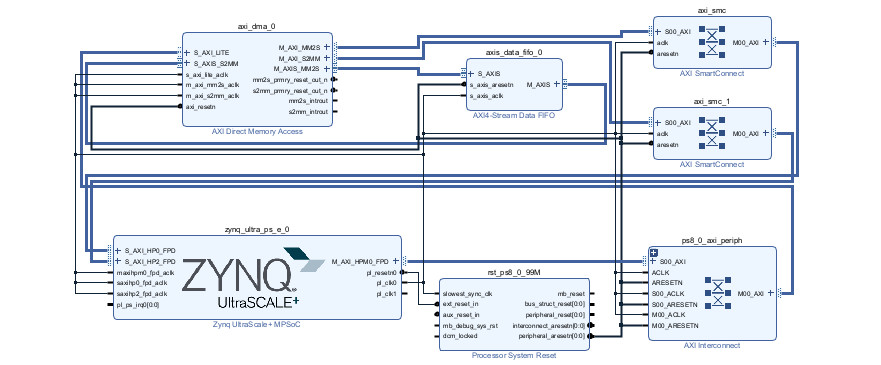
\includegraphics[width = 18cm]{picture/dma/z3976842715300_efb45c6db2d11f0ef02b16d20527631b.jpg}
    \caption{Block Design of DMA transferring}
    \medskip
\end{figure}
In Fig. 3.12, this is an example of communication between PS-PL. There is an array of data in DRAM with 32-bit elements. This array will be transferred to FIFO in PL through DMA channel. FIFO plays a role as a send and receive channel which creates a loop back. On the PS side, we can easily modify the input of the array.
\begin{lstlisting}[language = Python]
    from pynq import Overlay
    from pynq import allocate
    import numpy as np
    ol = Overlay("./KRIA_KV260_DMA.bit")

    dma = ol.axi_dma_0
    dma_send = ol.axi_dma_0.sendchannel
    dma_recv = ol.axi_dma_0.recvchannel

    data_size = 1000
    input_buffer = allocate(shape=(data_size,), dtype=np.uint32)

    for i in range(data_size):
        input_buffer[i] = i + 0xcafe0000
    for i in range(10):
        print(hex(input_buffer[i]))

    dma_send.transfer(input_buffer)
    output_buffer = allocate(shape=(data_size,), dtype=np.uint32)
    for i in range(10):
        print('0x' + format(output_buffer[i], '02x'))
    dma_recv.transfer(output_buffer)
    for i in range(10):
        print('0x' + format(output_buffer[i], '02x'))
\end{lstlisting}
\subsection{PYNQ AXI CDMA to BRAM}
BRAM is used to store images and kernels in PL. IP Block Memory Generator is used in this case. Because DMA use AXI interface and Block Memory Generator does not, so we need AXI BRAM controller to transfer between BRAM and DMA.

To use AXI CDMA IP, designers must understand how to configure IP’s registers and modify the master base address in order to locate data due to each purpose.
\begin{figure}[H]
    \centering
    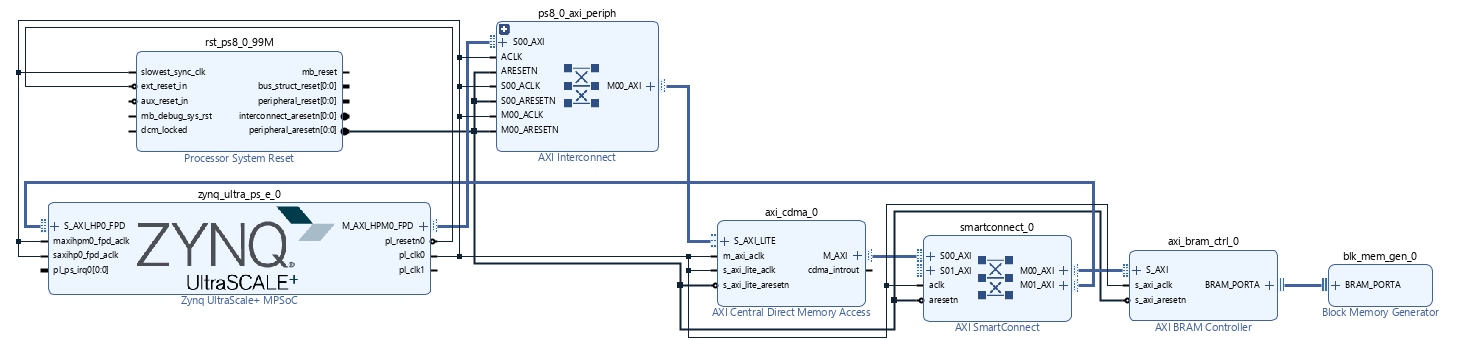
\includegraphics[width = 18cm]{picture/dma/one bram.png}
 \caption{Block Design of CDMA and one BRAM}
    \medskip
\end{figure}

\begin{lstlisting}[language = Python]
    cdma = overlay.axi_cdma_0
    input_buffer = allocate(shape=(1024,), dtype=np.uint32)
    output_buffer = allocate(shape=(1024,), dtype=np.uint32)
    for i in range(1024):
        input_buffer[i] = i

    start_time = time.time()
    transfer(cdma, input_buffer.physical_address, 0xE000_0000, 1024*4)
    transfer(cdma, 0xE000_0000, output_buffer.physical_address, 1024*4)
    end_time = time.time()

    print("%s seconds" % (end_time - start_time))
    print()
    print(output_buffer)
\end{lstlisting}
\begin{lstlisting}
    Transferring...
    Transfered 256 bytes from 634380288 to 3758096640
    CDMA Done.
    Transferring...
    Transfered 256 bytes from 3758096640 to 448798720
    CDMA Done.
    0.002915620803833008 seconds
    ...
\end{lstlisting}

So, the above example is for one BRAM. However, in the realistic problem, we need to handle a large amount of data. Using one BRAM cannot store those amount and also slow down the efficiency of hardware processing and optimization. Therefore, there is a method which is using multiple BRAMs at the same time to store data with corresponding base address and range.

We will discuss 2 ways of transferring data to 4 BRAMs by using CDMA.
\begin{figure}[H]
    \centering
    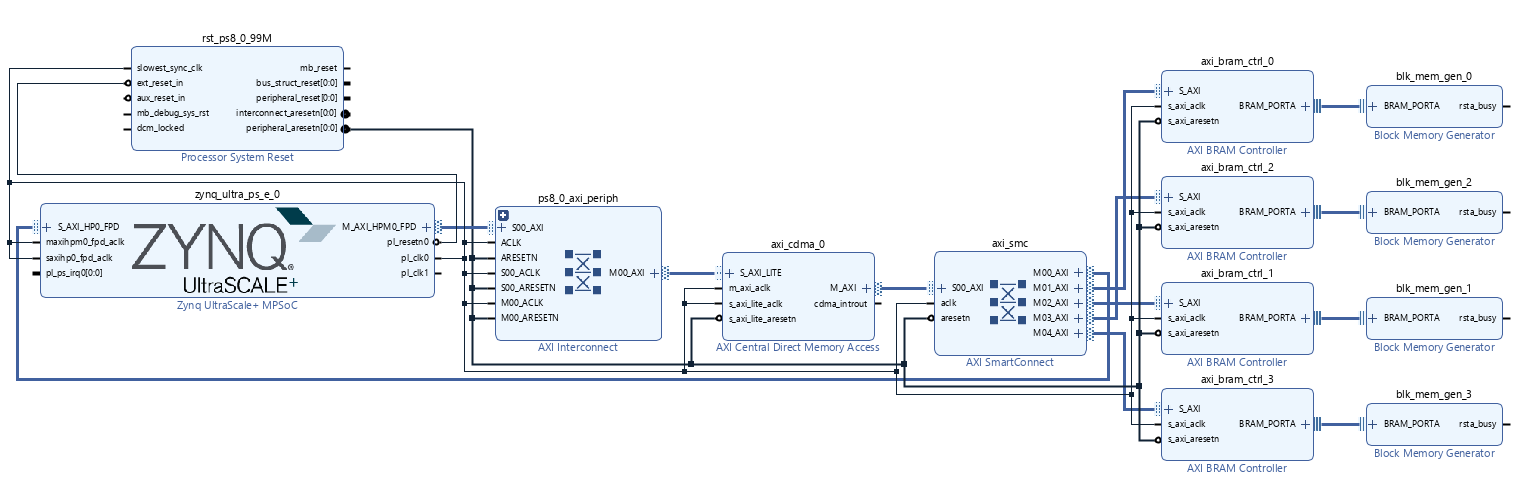
\includegraphics[width = 16cm]{picture/dma/bramtransfer.png}
    \caption{Block Design of CDMA and 4 BRAMs}
\end{figure}

\begin{lstlisting}
    input_buffer0 = allocate(shape=(2048,), dtype=np.uint32)
    input_buffer1 = allocate(shape=(2048,), dtype=np.uint32)
    input_buffer2 = allocate(shape=(2048,), dtype=np.uint32)
    input_buffer3 = allocate(shape=(2048,), dtype=np.uint32)

    output_buffer0 = allocate(shape=(2048,), dtype=np.uint32)
    output_buffer1 = allocate(shape=(2048,), dtype=np.uint32)
    output_buffer2 = allocate(shape=(2048,), dtype=np.uint32)
    output_buffer3 = allocate(shape=(2048,), dtype=np.uint32)
    
    for i in range(2048):
        input_buffer0[i] = i
        input_buffer1[i] = i+2048
        input_buffer2[i] = i+2048*2
        input_buffer3[i] = i+2048*3

    transfer(cdma, input_buffer0.physical_address, 0xE000_0000, 2048*4)
    transfer(cdma, 0xE000_0000, output_buffer0.physical_address, 2048*4)

    transfer(cdma, input_buffer1.physical_address, 0xE200_0000, 2048*4)
    transfer(cdma, 0xE200_0000, output_buffer1.physical_address, 2048*4)

    transfer(cdma, input_buffer2.physical_address, 0xE400_0000, 2048*4)
    transfer(cdma, 0xE400_0000, output_buffer2.physical_address, 2048*4)

    transfer(cdma, input_buffer3.physical_address, 0xE600_0000, 2048*4)
    transfer(cdma, 0xE600_0000, output_buffer3.physical_address, 2048*4)

\end{lstlisting}

The first method is transferring data in the parallel way which means pushing data into 4 arrays at the same time and same amount. We set the master base address at default. The benefit of this method is fast and independent between each buffer. 
\begin{figure}[H]
    \centering
    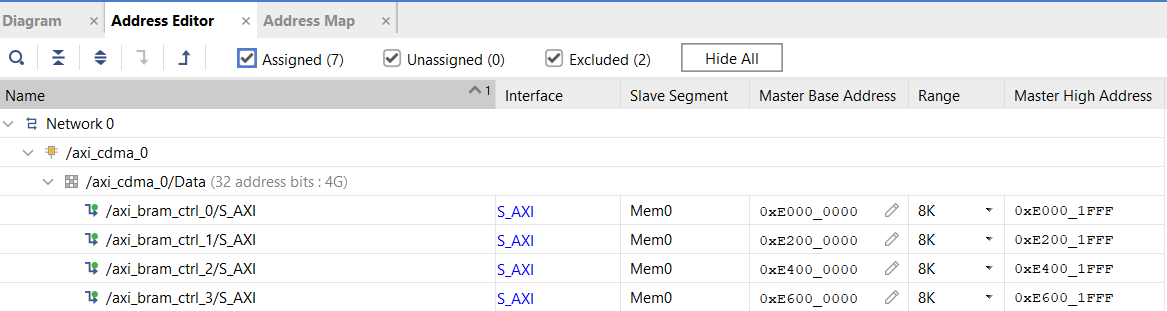
\includegraphics[width = 16cm]{picture/dma/Screenshot 2022-12-23 072354.png}
    \caption{Address Editor for Sequential 4 BRAMs}
\end{figure}
\begin{lstlisting}
    input_buffer0 = allocate(shape=(2048*4,), dtype=np.uint32)
    output_buffer0 = allocate(shape=(2048*4,), dtype=np.uint32)
    for i in range(2048*4):
        input_buffer0[i] = i

    transfer(cdma, input_buffer0.physical_address, 0xE000_0000, 2048*4*4)
    transfer(cdma, 0xE000_0000,output_buffer0.physical_address, 2048*4*4)
\end{lstlisting}

In the second method, we want to connect 4 BRAMs to be a sequential chain. Therefore, we need to modify the memory map of each BRAM, starting by BRAM0.

\section{One Dimensional Convolution}
\subsection{Data flow}
With 1D Convolution, assume that we have to compute data is an array with k elements (called input\_data[k]) with a kernel is array with 3 elements (called ker[3]). First we prepare the input data and the kernels required for the computation through the PS. The PS will then load the provided materials to the CDMA using AXI streaming. And the CDMA will push data into PL, using AXI streaming, through AXI BRAM controller and store it in 4 BRAMs. 

The way to store input data must follow the rule: the first BRAM stores input\_data[0] to input\_data[k/4+2]; the second BRAM stores input\_data[k/4] to input\_data[2k/4+2]; the third BRAM stores input\_data[2k/4] to input\_data[3k/4+2]; the fourth BRAM stores input\_data[3k/4] to input\_data[k]. And with the same way, kernel will be loaded into a BRAM through CDMA, AXI BRAM controller using AXI streaming. 

After that, data and kernel will be loaded into Computing Core and stored in 5 FIFOs (data in 4 BRAMs will be loaded into 4 input FIFOs, kernel will be loaded into a kernel FIFO). Computing Core will operate the convolution and store the result in 4 BRAMs. AXI will then be used again to transfer the result to the CDMA, and from which is loaded back to the PS for result displaying.
\begin{figure}[H]
    \centering
    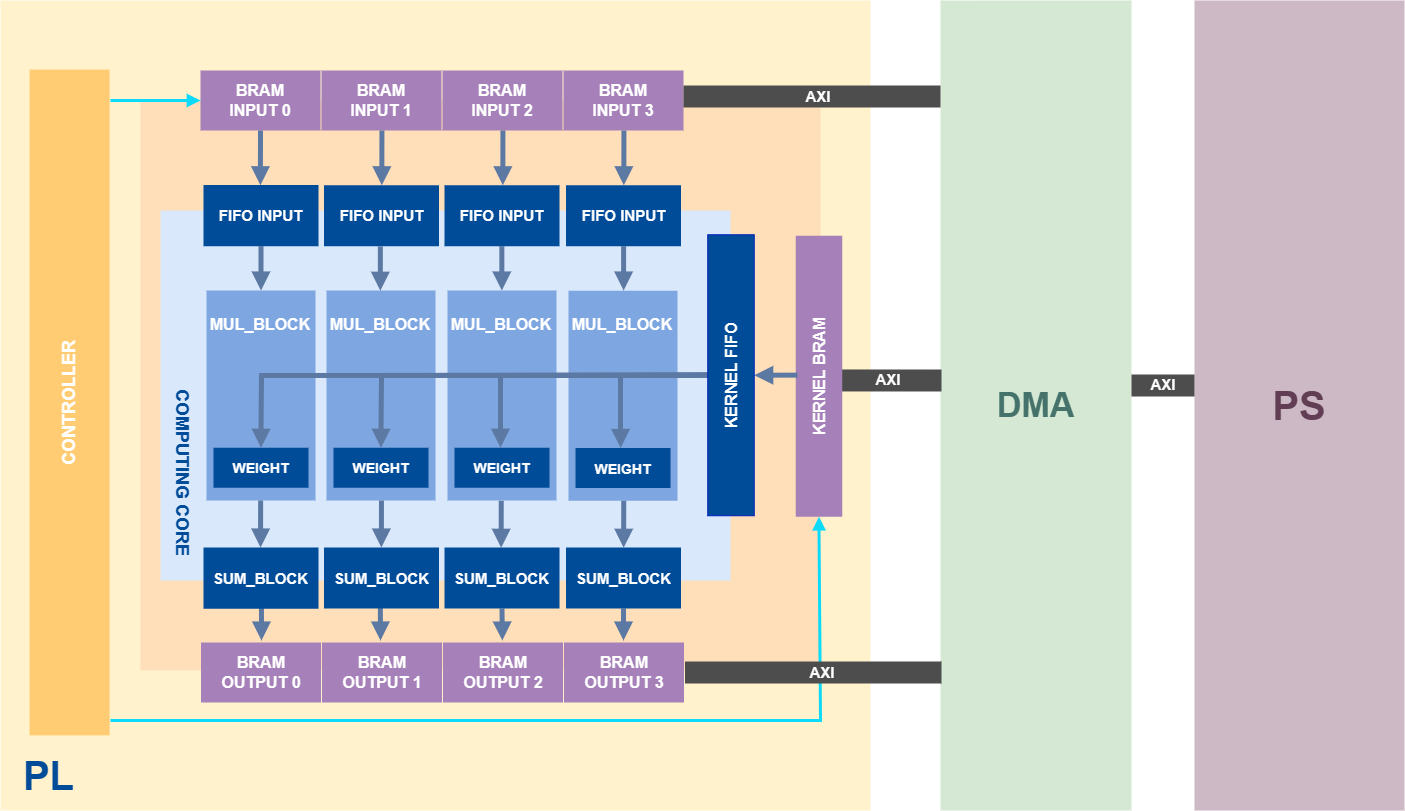
\includegraphics[width = 12cm]{picture/Computing Core/convo_dataflow.drawio.png}
    \caption{Data flow}
    \medskip
\end{figure}

\subsection{Computing Core}
As stated before, the computing core is an essential part of the PL, taking on computing a unit of convoluted operation. The computing core contains 5 FIFOs, in which, all of the input array and kernel is stored. In each 3 cycles, group of 3 data of each FIFO INPUT is routed to multiply with the weights of kernels transferred in by the Kernel FIFO (the process happens in MUL\_BLOCK). After being multiplied, the results then be sent to SUM\_BLOCK to be summed up. The final result of Computing Core is 4 elements that corresponds to 4 elements of the 1D Convolution operation. 
\begin{figure}[H]
    \centering
    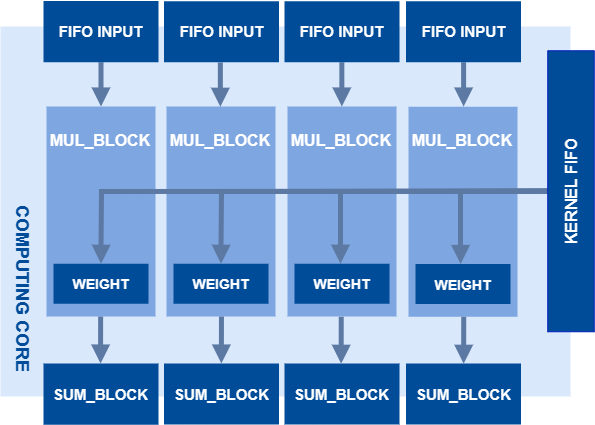
\includegraphics[width = 8cm]{picture/Computing Core/convo_dataflow-Page-2.drawio.png}
    \caption{Computing Core}
    \medskip
\end{figure}
\chapter{Result}
\section{DMA Transferring Time}
This section is about a survey of transferring four blocks of data from the kernel to 4 BRAMs (the
first block is transferred to BRAM0, the second block is transferred to BRAM1, the third block is
transferred to BRAM2, the last block is transferred to BRAM3). Each BRAM is 8KB in size and contiguous in address; each data block is 8KB in size. There are two methods of transferring:\\

\textbf{First method - 4 shot transfer } Transfer each data block into each BRAM, which means there
are 4 DMA transfers. Each transfer will move 8KB of data to a single BRAM. In total, DMA will
transfer 4*8KB data.\\

\textbf{Second method - 1 shot transfer } DMA will transfer one block of data by push data into the first BRAM buffer due to the sequential Master Base Address which has the structure as [8KB meaningful data - 8KB meaningful data - 8KB meaningful data - 8KB meaningful data]. The meaningful data block is one of 4 blocks we want to transfer to BRAM. In total, DMA
will transfer 4*8KB data.

\begin{figure}[H]
    \centering
    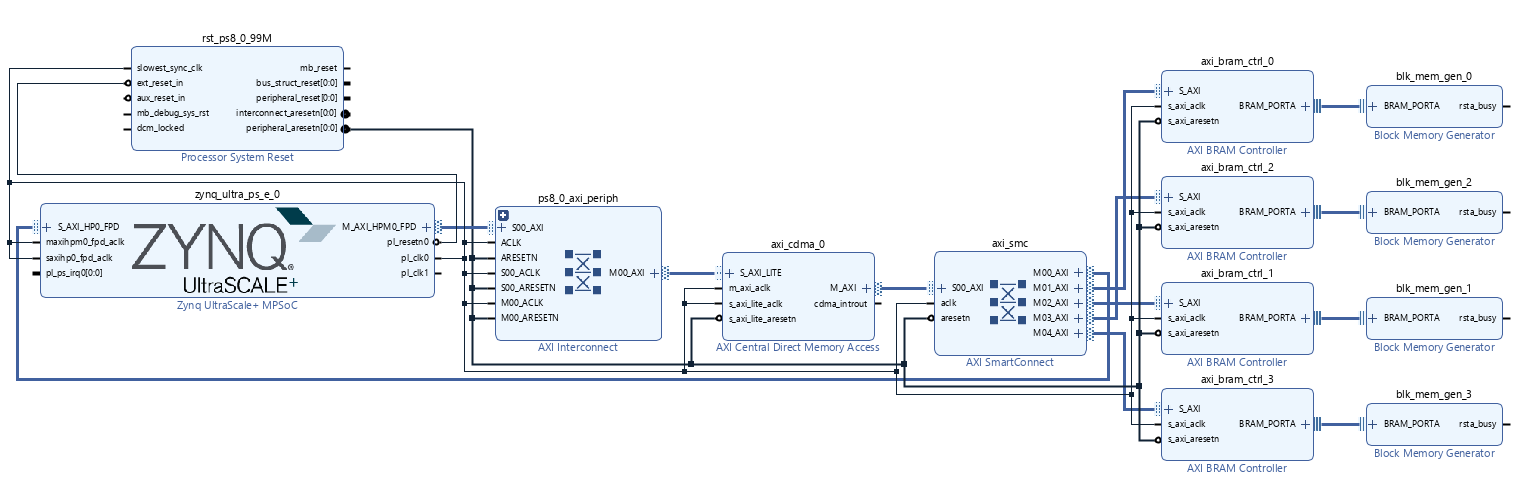
\includegraphics[width = 16cm]{picture/dma/bramtransfer.png}
    \caption{Block design for CDMA transferring time survey}
    \medskip
\end{figure}

\textbf{Result}  Although in 1-shot transfer, amount of data is four times larger than 4-shot transfer, the 1-shot transfer is still about 9.3 times faster than 4-shot transfer. This is because each time program start a DMA transfer, it costs lots of clock cycles to configure the register to be ready for a transfer.

\section{FIFO Testbench}
In this section, we send data into FIFO sequentially from 0 to 16; and we have 2 signals to control read and write process are readsignal and writesignal. Data is loaded into FIFO only when writesignal active high; Data is read out of FIFO only when readsignal active high.

\begin{figure}[H]
    \centering
    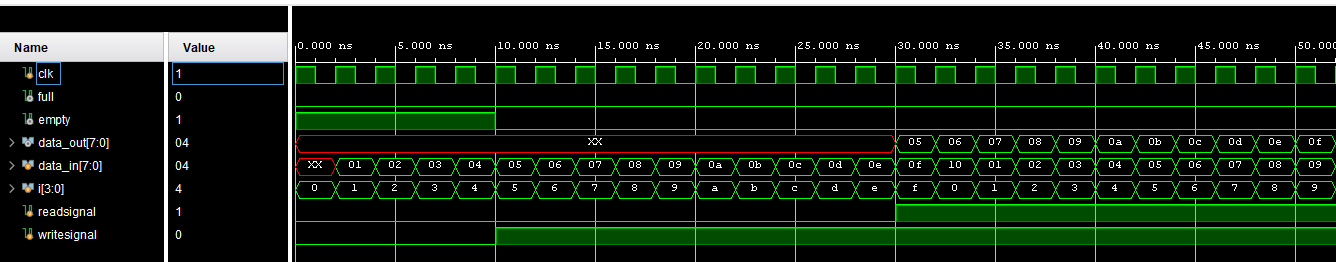
\includegraphics[width = 16cm]{picture/result/FIFO/waveformFIFOpng.png}
    \caption{FIFO Waveform}
    \medskip
\end{figure}

In this waveform, we can see at 10ns, writesignal active high, and data comes into FIFO is 0x05; after a clock cycle, data comes into FIFO is 0x06,... At 30ns, readsignal active high, and data comes out FIFO is the first data came into FIFO; after a clock cycle, data comes out FIFO is the second data came into FIFO,...

\section{Adder/Subtracter IP Testbench}
In this section, we set IP in add mode; inputs are unsigned type and width is 4 bits; Latency is 1. 

Therefore, the result is showed immediately when input received data.
\begin{figure}[H]
    \centering
    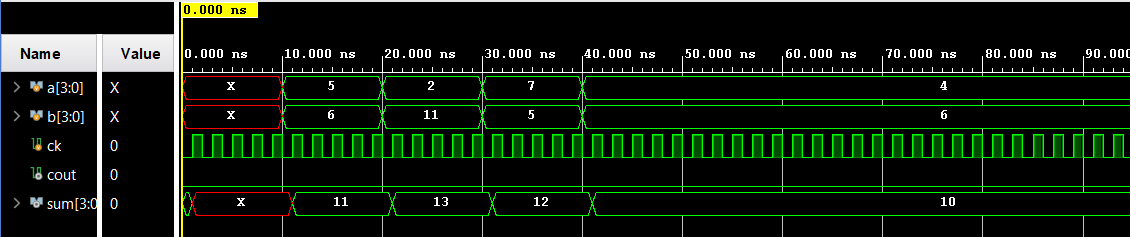
\includegraphics[width = 16cm]{picture/result/add/waveformADD.png}
    \caption{Adder/Subtracter IP Waveform}
    \medskip
\end{figure}

\section{Multiplier IP Testbench}
In this section, we set inputs are signed type and width is 8 bits; output width in auto mode, so that the width is 16 bits. Pipeline stages is 3.

Therefore, the result is showed after 3 clock cycle when input received data.

\begin{figure}[H]
    \centering
    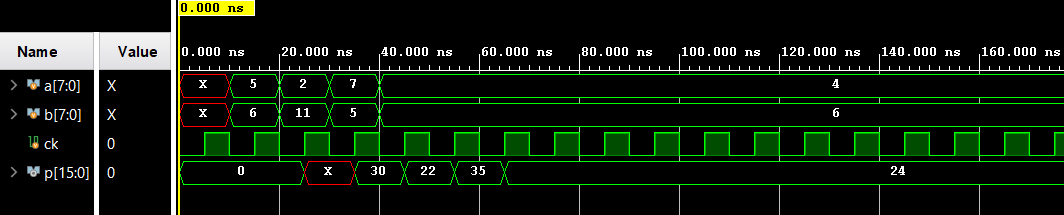
\includegraphics[width = 16cm]{picture/result/mul/waveformMUL.png}
    \caption{Multiplier IP Waveform}
    \medskip
\end{figure}

\section{Floating-point IP Testbench}
In this section, we set IP in add mode, blocking mode, and maximum latency (latency is 12), and the with of input is 32 bits.\\

\begin{figure}[H]
    \centering
    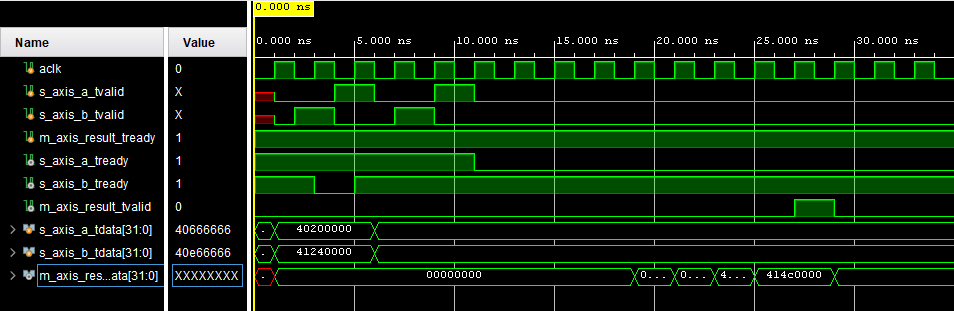
\includegraphics[width = 16cm]{picture/result/float/waveformfloating.png}
    \caption{Floating-point IP Waveform}
    \medskip
\end{figure}

In this waveform, we can see at 2ns, s\_axis\_b\_tvalid active high; and the input of b chanel is stored. And at 4ns, when s\_axis\_b\_tvalid active high, the operation started, and after 12 clock cycles, s\_axis\_result\_tvalid active high to inform that operation has done.
\section{Computing Core Testbench}
In this section, we tested a single data path of computing core.

\begin{figure}[H]
    \centering
    \includegraphics[width = 4cm]{picture/result/computingcore/convo_dataflow-Page-3.drawio.png}
    \caption{Data path of Computing Core is tested}
    \medskip
\end{figure}

In this test, the array input is data\_in\_0[16] = \{0, 1, 2, 3, 4, 5, 6, 7, 8, 9, 10, 11, 12, 13, 14, 15\}; kernel is data\_kernel[3] = \{1, 2, 3\}. Done signal active high when output is ready, en signal active high when there is a data loaded into FIFO INPUT.

\begin{figure}[H]
    \centering
    \includegraphics[width = 12cm]{picture/result/computingcore/convo_dataflow-Page-4.drawio.png}
    \caption{Demonstrate the computation}
    \medskip
\end{figure}

\begin{figure}[H]
    \centering
    \includegraphics[width = 18cm]{picture/result/computingcore/computingcoretb.png}
    \caption{Waveform of data path which is tested}
    \medskip
\end{figure}
\begin{lstlisting}[language= verilog]  
    initial begin
        #6 reset = 0;
        #1 reset = 1;
    end
    
    always @(posedge clk or negedge reset)
    begin
        if (!reset)
        begin
            i <= 0;
            j <= 1;
            data_in_0 <= data[0];
        end
        else
        begin
            if ((i < 3))
            begin
                data_kernel = kernel [i];
                i <= i + 1;
            end
            
            if (j < 15 && en == 1)
            begin
                data_in_0 <= data [j];
                j <= j + 1;
            end
        end
    end
\end{lstlisting}

\chapter{Conclusion}
The project is mainly in its early stage, and we are working hard to bring out the finest IP core possible. Nevertheless, we have finished constructing some crucial parts and modules regarding FPGA implementation. Most of the implementations have been carried out and tested using Vivado simulation, while some have been implemented on Kria-Ubuntu OS by using PYNQ Jupyter Notebook. The rest will be built later, along with a detailed system statistic.

Our plan is to design the complete computing core with communication interface (BRAM) and the block design. After that, we will start to implement the data flow that we have suggested before.

\appendix
\chapter{PYNQ Environment Setup}

Unlike common PYNQ supported Xilinx boards installation images, Kria PYNQ installation requires three primary steps:\cite{hackster.io}
\begin{itemize}
    \item Download and install the KV260 Ubuntu image and boot to the Ubuntu-desktop.
    \item Clone the PYNQ framework to the Ubuntu desktop home folder and install the framework.
    \item Run the JupyterLab from the web browser.
\end{itemize}
\textbf{Step 1:}
\begin{itemize}
    \item The Kria KV260 starter kit - supported Ubuntu 20.04.3 LTS image can be downloaded from the link: https://ubuntu.com/download/amd-xilinx and using Balena Etcher or a similar imaging application, write the download image file to an SD Card.
    \item Insert the boot image in the card slot J11 on the Kria KV260 board. Connect an HDMI/Displayport monitor, keyboard and mouse. Connect ethernet cable for internet connection and power supply to the DC jack.
    \item Power ON the board and wait until Kria boots into the Ubuntu login page. Ubuntu precompiled boot image will ask to change the default password and log in
    \item Since installing the PYNQ Jupyter environment done, we need to install the Xilinx system management snap package using the following code:
\end{itemize}
\begin{lstlisting}
    sudo snap install xlnx-config --classic
    \end{lstlisting}
    Note: Xilinx Gstreamer package configuration. Do not use, in this instance. Installing the Gstreamer environment seems to break the PYNQ installation.
    \begin{lstlisting}
    # DO NOT USE
    xlnx-config.sysinit
    \end{lstlisting}

\textbf{Step 2:}
\begin{itemize}
    \item Clone the PYNQ framework from GitHub using the terminal and access the PYNQ directory.
    \item Once in the directory, run the bash script to install the PYNQ package.
    \begin{lstlisting}
    git clone https://github.com/Xilinx/Kria-PYNQ.git
    cd Kria-PYNQ
    sudo bash install.sh
    \end{lstlisting}
\end{itemize}

\textbf{Step 3:}\\

Now we can access the PYNQ Jupyter Lab directly using the Kria desktop web browser or access from another computer by using the URL IP address or namespace\\

\textbf{Note:}
\begin{itemize}
    \item If lost internet connection while installing, we have to open install.sh file to install from error part.
    \item At this time, we can't use the newest Ubuntu version because it has not support yet. And when installation complete, despite of the suggestion of the system, we must not upgrade to the newest version.
\end{itemize}

\chapter{Some tutorials for using PYNQ Framework}
\includepdf[page=-]{PYNQ-GS-GPIO (2).pdf}
\includepdf[page=-]{KRIA-KV260-PYNQ-DMA.pdf}
\clearpage
\addcontentsline{toc}{chapter}{Bibliography}
\printbibliography


\end{document}

